\documentclass[12pt,a4paper]{article}

% Paket för svenska
\usepackage[utf8]{inputenc}
\usepackage[swedish]{babel}
\usepackage[T1]{fontenc}
\usepackage{float}
% övriga paket
\usepackage{graphicx}
\usepackage{hyperref}
\usepackage{cite}
\usepackage{setspace}
\usepackage{geometry}
\usepackage{fancyhdr}
\usepackage{parskip}
% Sidlayout
\geometry{margin=2.5cm}
\onehalfspacing

% Sidhuvud och sidfot
\pagestyle{fancy}
\fancyhf{}
\rhead{\thepage}
\lhead{\leftmark}
\renewcommand{\headrulewidth}{0.4pt}

\begin{document}

% Framsida
\begin{titlepage}
    \centering

    \vspace*{2cm}

    
\includegraphics[width=0.3\textwidth]{miun_logo.png}

    \vspace{1cm}

    {\huge\bfseries Brewmaster Coffee UI/UX\par}
    \vspace{0.5cm}
    {\large Rethinking and Developing the Design Behind Premium Coffe-Machine Interfaces \par}

    \vspace{2cm}

    {\Large
    Elias Danielsson (elda2203@student.miun.se)\\
    Erik Sawander (ersa@student.miun.se)\\
    Theodor Christensen (thch2100@student.miun.se)\\
    Victor Hillström(vihi2200@student.miun.se)\\
    }

    \vspace{1cm}

    {\large Gruppnummer: 3\par}

    \vfill

    {\large
    Program: [TDTEA]\\
    Kurs: DT168G Människa-datorinteraktion\\
    Examinator: Jimmy Åhlander\\
    Mittuniversitetet\\
    \today
    }

\end{titlepage}

\newpage

% Sammanfattning
\section*{Sammanfattning}
\addcontentsline{toc}{section}{Sammanfattning}

Sammanfattningen ska beskriva hela rapporten kortfattat på cirka 250 ord. Den ska täcka:
\begin{itemize}
    \item Bakgrund och syfte med projektet
    \item Vilka metoder som användes
    \item De viktigaste resultaten
    \item Huvudsakliga slutsatser
\end{itemize}

\textit{[Här skriver du din sammanfattning. Kom ihåg att detta är en separat text som ska kunna läsas fristående från resten av rapporten. En läsare ska kunna få en helhetsbild av hela projektet bara genom att läsa sammanfattningen.]}

\vspace{1cm}

\noindent\textbf{Nyckelord:} Interaktionsdesign, användbarhet, användarcentrerad design, [lägg till relevanta nyckelord]

\newpage

% Innehållsförteckning
\tableofcontents
\newpage

% Kapitel
\section{Inledning}

I takt med att kaffekulturen växer börjar allt fler intressera sig för att brygga kaffe av kvalitet hemifrån. Dagens kaffemaskiner är ofta utrustade med avancerade funktioner som låter användaren i detalj skräddarsy sin kaffebryggning. Detta medför komplexa utmaningar inom användbarhet och tillgänglighet. 

\subsection{Bakgrund}

Efterfrågan om att kunna kontrollera små variabler som vattenpulsintervaller, malningsgrad, vattentemperatur och bryggningstid har ökat hos premium-kaffemaskiner. Denna utveckling skapar en svårighet i att skapa en bra användarupplevelse för alla användare. Ena sidan är användare som enkelt och snabbt vill kunna brygga en kopp kaffe och andra sidan entusiaster som vill ha full kontroll över alla bryggvariabler.

Många av dagens kaffemaskiner tenderar att inrikta sitt användargränssnitt till det extrema. Antingen genom att gömma avancerade funktioner eller att exponera alla detaljer. Att hitta balansen mellan enkelhet och djup funktionalitet är svårt och något som få maskiner lyckas med. Vanliga användbarhetsproblem som förekommer:

\begin{itemize}
    \item Menystrukturer med komplexa undermenyer
    \item Saknad tydlighet om vad parametrar gör
    \item Svårigheter att återanvända exakta inställningar
    \item Begränsade möjligheter till personalisering
\end{itemize}

Genom att använda principer från interaktionsdesign och användarcentrerad design kan man skapa ett gränssnitt som gör detaljerad kaffebryggning tillgängligt för en större målgrupp utan att förlora efterfrågade funktioner. 

\subsection{Syfte}

Syftet med projektet är att förbättra användarupplevelsen av avancerade kaffemaskiner genom skapandet av ett gränssnitt som tilltalar både nybörjare och erfarna kaffeentusiaster samtidigt som den sänker inlärningströskeln.  

Projektet syftar till att utforska hur ett profilsystem kan användas för att undanhålla komplexitet på ett sätt så användare själv kan anpassa komplexitetsnivån utifrån intresse.

\subsection{Mål}

Projektets mål är att leverera:

\begin{itemize}
    \item En högfidelitetsprototyp av ett touchbaserat gränssnitt för en premium-kaffemaskin som balanserar enkelhet med avancerade funktionaliteter.
    \item Ett profilbaserat system där användare kan:
    \begin{itemize}
        \item Brygga kaffe med förinställda profiler
        \item Skapa bryggprofiler med egna anpassade preferenser. 
        \item Anpassa avancerade inställningar (vattenpulsinervall, temperatur, malningsgrad och extraktionstid)
    \end{itemize}

    \item Personaliseringsfunktion i form av val av färgtema

    \item Dokumentation och utvärdering av designprocessen genom användarcentrerade metoder
    
\end{itemize}


\subsection{Avgränsningar}

Projektet avgränsas till följande:

\begin{itemize}
    
    \item \textbf{Plattform och implementation:} Projektet fokuserar på design av användargränssnittet (UX/UI). Funktioner kommer interaktivt vara funktionella med inte kopplade till praktisk funktionalitet. Inga back-end system kommer att implementeras.

    \item \textbf{Maskintyp:} Fjärrstyrning eller mobilapplikationer ingår inte i projektet. Fokus ligger på gränssnittet på kaffemaskinens touchskärm.

    \item \textbf{Språk:} För att förenkla utvecklingsprocessen presenteras avandargränssnittet endast på engelska.

    \item \textbf{Målgrupp:} Kaffeälskare med varierande erfarenhet av kaffebryggning som vill göra premium kaffe hemifrån.


\end{itemize}

\textbf{Motivering:} Projektets avgränsningar möjliggör att fokus kan ligga på användbarhet och interaktionsdesign utan att arbetet belastas av tekniska implementationer. Detta resulterar i en mer iterativ och användarcentrerad process inom given tidsram. 

\textbf{Potentiella konsekvenser:} Eftersom ingen backend-implementation utförs begränsas möjligheten till feedback kring responstider. Detta påverkar hur realistiskt användbarhetstesterna visar den faktiska produkten. 


\subsection{Arbetsfördelning}

Projektet genomförs som ett samarbete där alla gruppmedlemmar bidrar till designprocessen. Följande arbetsfördelning har etablerats:

\begin{table}[h]
\centering
\begin{tabular}{|l|p{9cm}|}
\hline
\textbf{Gruppmedlem} & \textbf{Ansvar och bidrag} \\
\hline
Elias Danielsson & Brainstorming design-idéer, prototyputveckling (initial fas), rapportskrivande (generell struktur, inledning), feedback insamling, merging av prototyper (Högnivå), förbättring av prototyp \\
\hline
Erik Sawander & Brainstorming design-idéer, prototyputveckling (initial fas), rapportskrivande(fill in later), feedback insamling, \\
\hline
Theodor Christensen & Prototyputveckling (initial fas), Skrivande av frågeformulär, rapportskrivande(fill in later), feedback insamling, \\
\hline
Victor Hillström & Prototyputveckling (initial fas), merging av prototyper (Lågnivå), rapportskrivande(fill in later), feedback insamling, \\
\hline
\end{tabular}
\caption{Arbetsfördelning i projektgruppen (uppdateras löpande under projektets gång)}
\end{table}

\newpage

\section{Teori}

\textit{[Teorikapitlet ska lyfta de teoretiska delar som är relevanta för ert arbete. Fokusera på koncept från kurslitteraturen och forskningsartiklar som är viktiga för just ert projekt. Teorikapitlet ska vara tungt refererat till tidigare arbeten.]}

\textit{[Kom ihåg: Behandla endast teori som är relevant för ert arbete. Ni skriver inte en lärobok, utan lyfter bara de delar som ni senare kommer att referera till i design, metod eller diskussion.]}


\subsection{Användarcentrerad design}

\textit{[Exempel på teorisektion]}

Användarcentrerad design (User-Centered Design, UCD) är en designfilosofi där användaren står i centrum genom hela utvecklingsprocessen \cite{sharp2019}. Metoden innebär att användarna aktivt involveras i designprocessen genom iterationer av design, test och revidering.

De fyra huvudprinciperna för användarcentrerad design är:
\begin{enumerate}
    \item Tidigt fokus på användare och uppgifter
    \item Empirisk mätning av produktanvändning
    \item Iterativ design
    \item Integrerad design
\end{enumerate}


\subsection{Användbarhet}

\textit{[Beskriv relevanta användbarhetsbegrepp]}

Nielsen definierar användbarhet genom fem komponenter \cite{nielsen2012}:
\begin{itemize}
    \item \textbf{Lärbarhet}: Hur lätt är det för användare att utföra grundläggande uppgifter första gången?
    \item \textbf{Effektivitet}: När användarna lärt sig designen, hur snabbt kan de utföra uppgifter?
    \item \textbf{Minnesvärdhet}: När användare återkommer efter en period, hur lätt återupprättar de kompetensen?
    \item \textbf{Fel}: Hur många fel gör användare, hur allvarliga är de, och hur lätt kan de återhämta sig?
    \item \textbf{Tillfredsställelse}: Hur trevlig är designen att använda?
\end{itemize}


\subsection{Forskningsetiska principer}

\textit{[Detta är obligatoriskt att inkludera]}

I projekt som involverar människor är det viktigt att följa Vetenskapsrådets forskningsetiska principer \cite{vetenskapsradet2002}. De fyra huvudkraven är:

\begin{itemize}
    \item \textbf{Informationskravet}: Forskaren ska informera deltagare om forskningens syfte
    \item \textbf{Samtyckeskravet}: Deltagare har rätt att själva bestämma över sin medverkan
    \item \textbf{Konfidentialitetskravet}: Uppgifter om deltagare ska förvaras på ett sätt så obehöriga inte kan ta del av dem
    \item \textbf{Nyttjandekravet}: Insamlade uppgifter får endast användas för forskningsändamål
\end{itemize}


\subsection{[Lägg till fler teorisektioner efter behov]}

\textit{[Till exempel: Gestaltlagar, designprinciper, prototypmetoder, evalueringsmetoder, etc.]}

\newpage

\section{Metod}

\subsection{Övergripande tillvägagångssätt}

\textit{[Beskriv er designprocess på en övergripande nivå]}

Projektet följde en iterativ användarcentrerad designprocess med följande huvudsteg:
\begin{enumerate}
    \item Målanalys och kravfångst
    \item Designalternativ och prototyper
    \item Utvärdering med målgruppen
\end{enumerate}

Totalt genomfördes [X] iterationer där designen förfinades baserat på feedback från användare.


\subsection{Iteration 1: Kravfångst och målanalys}

Baserat på tidigare erfarenheter av målgruppen och kaffemaskiner så bestämdes mål och krav. Samt analyserades befintliga lösningar för bristar.  

\subsubsection{Personas}

Baserat på tidigare erfarenheter skapades 3 personas som representerar huvudsakliga användargrupper (se Bilaga B). %MARK we need our interviews to somewhat match our personas, the third one is whatever, thats just made up shit. 


\subsection{Iteration 2: Prototyputveckling}

\subsubsection{Lo-fi prototyper}


Initialt skapades pappersprototyper och digitala skisser (lo-fi) för att snabbt kunna utforska olika designalternativ. Detta tillvägagångssätt valdes eftersom det möjliggör snabb iteration och enkelt kan kastas vid behov \cite{sharp2019}.

\textbf{Design Studio:} Gruppen genomförde en design studio-session där varje gruppmedlem skissade ett lösningsförslag var. Förslagen diskuterades och de mest lovande idéerna kombinerades. 



\subsubsection{Hi-fi prototyper}

Efter validering av lo-fi prototyper utvecklades en högfidelitetsprototyp med hjälp av html css och javascript. Prototypen inkluderade sammansatta egenskaper från lo-fi prototyperna utefter design studio resultaten.


\subsection{Iterationer : Utvärdering} % do this as we go 

\subsubsection{Användbarhetstester}

\textit{[Detta är obligatoriskt att inkludera i minst en iteration]}

För att utvärdera prototypens användbarhet genomfördes användbarhetstester med [antal] deltagare från målgruppen.

\textbf{Testupplägg:} Testerna baserades på task-based usability testing. Deltagarna fick genomföra följande uppgifter:
\begin{enumerate}
    \item Brygg en kopp kaffe
    \item Skapa en profil 
    \item Schemalägg en bryggning
    \item Skapa en profil med malningsstorlek "fine"
\end{enumerate}

\textbf{Datainsamling:} Under testerna observerades och dokumenterades:
\begin{itemize}
    \item Tid för att genomföra uppgifter
    \item Antal fel och var de uppstod
    \item Deltagarnas kommentarer (think-aloud)
    \item Ålder 
    \item Subjektiv svårighet av uppgifterna 
    \item Framgång av att utföra navigation på första försöket 
    \item Om det saknades funktionalitet
\end{itemize}

\textbf{Analysmetod:} Data analyserades genom de kvantitativa metoderna felfrekvensanalys, och deskriptiv analys, samt de kvalitativa metoderna think-aloud protokollanalys, och kategorisering av användbarhetsproblem .

\subsection{Motivering av metodval}

De valda metoderna motiveras av att de tillsammans ger en helhetsbild av användarnas behov och hur väl designen möter dessa. Intervjuerna gav kvalitativ insikt i användarnas kontext, medan användbarhetstesterna mätte konkret användbarhet.

\newpage

\section{Design}

\subsection{Designkoncept}
% VICTOR do this 
\textit{[Beskriv det övergripande designkonceptet]}

Det övergripande designkonceptet baseras på [beskriv huvudidé]. Gränssnittet riktar sig till [målgrupp] och ska främst stödja [huvudsakliga uppgifter].

Designen följer principerna om [t.ex. visibility, feedback, constraints från kurslitteraturen] för att säkerställa god användbarhet.


\subsection{Iteration 1: Tidiga skisser}

I den första iterationen skapades flera olika designalternativ. Figur \ref{fig:tidiga_skisser}, \ref{fig:tidiga3} och \ref{fig:tidiga_2} visar exempel på tidiga pappersprototyper.

\begin{figure}[H]
    \centering
    \includegraphics[width=0.8\textwidth]{bilder/paper.png}
    \caption{Tidig pappersprototyper från design studio-sessionen}
    \label{fig:tidiga_skisser}
\end{figure}

\begin{figure}[H]
    \centering
    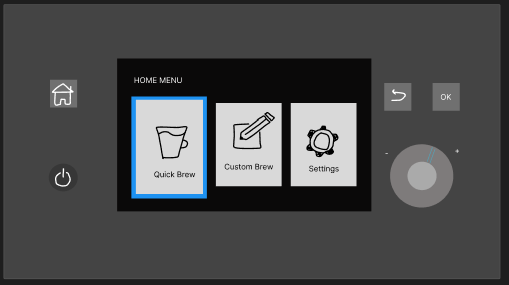
\includegraphics[width=0.8\textwidth]{bilder/victor1.png}
    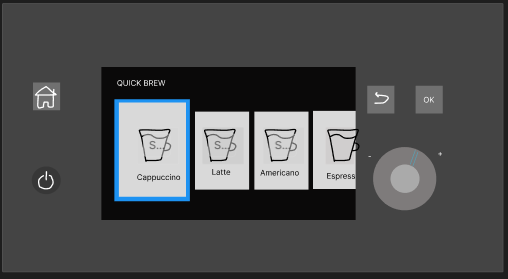
\includegraphics[width=0.8\textwidth]{bilder/victor2.png}
    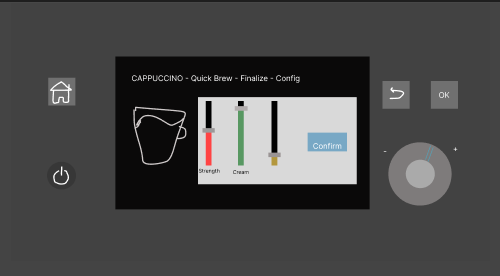
\includegraphics[width=0.8\textwidth]{bilder/victor3.png}
    \caption{Tidig prototyp från design studio-sessionen}
    \label{fig:tidiga_2}
\end{figure}

\begin{figure}[H]
    \centering
    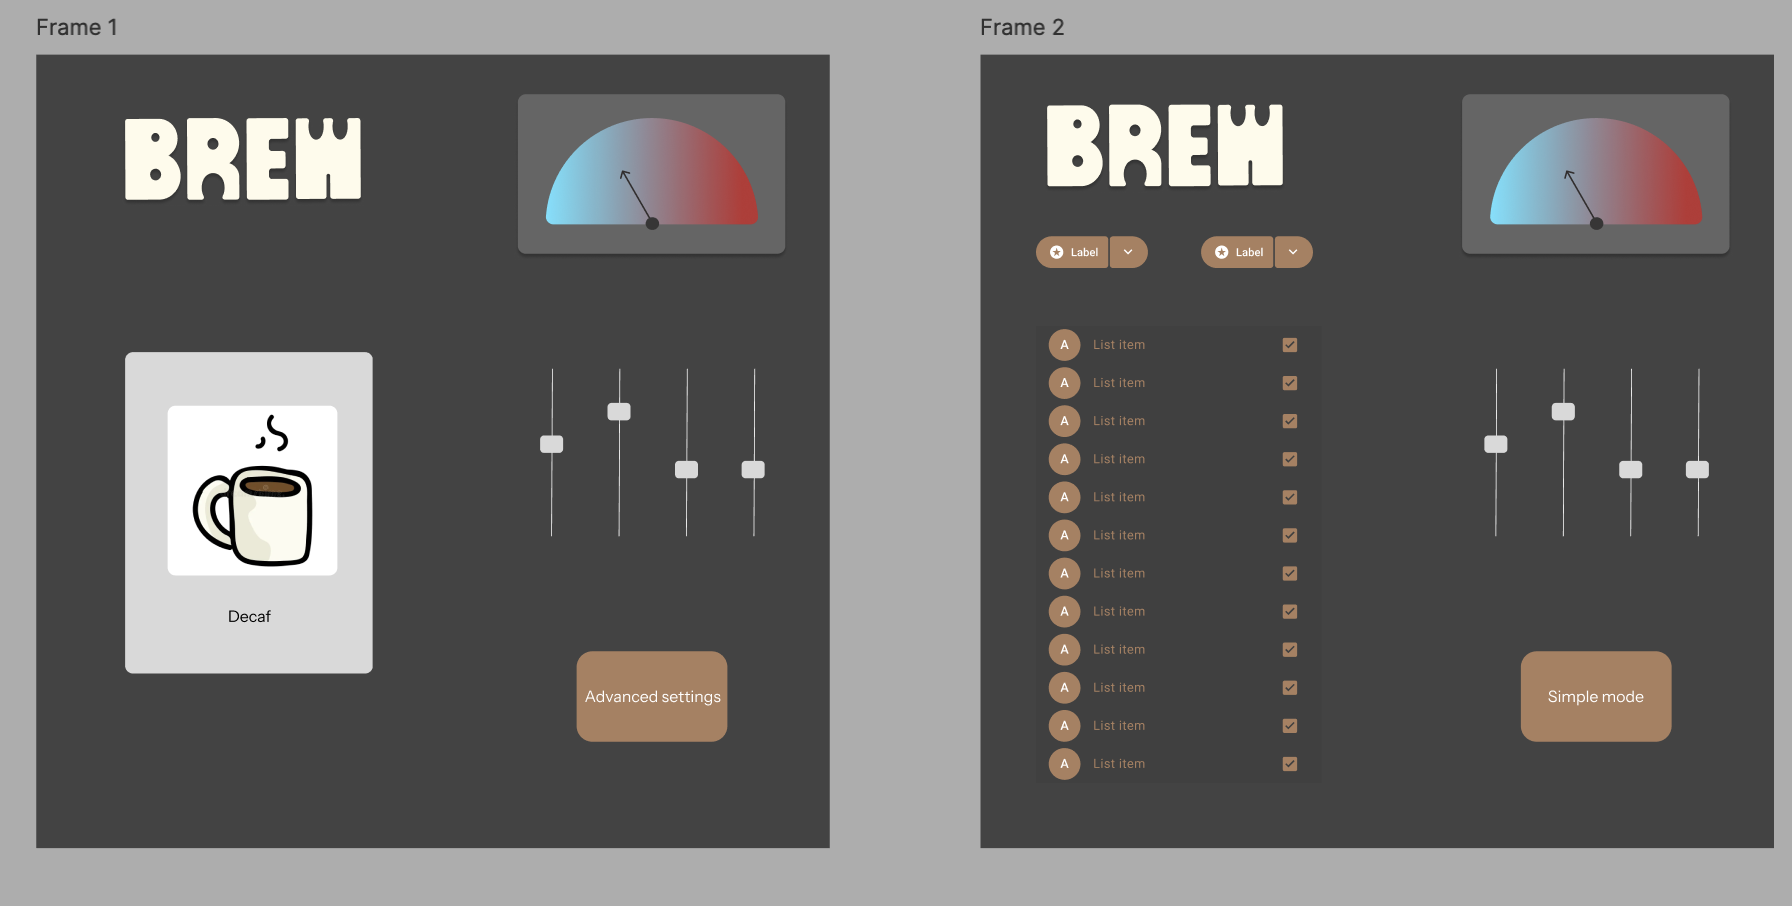
\includegraphics[width=0.8\textwidth]{bilder/sjov.png}
    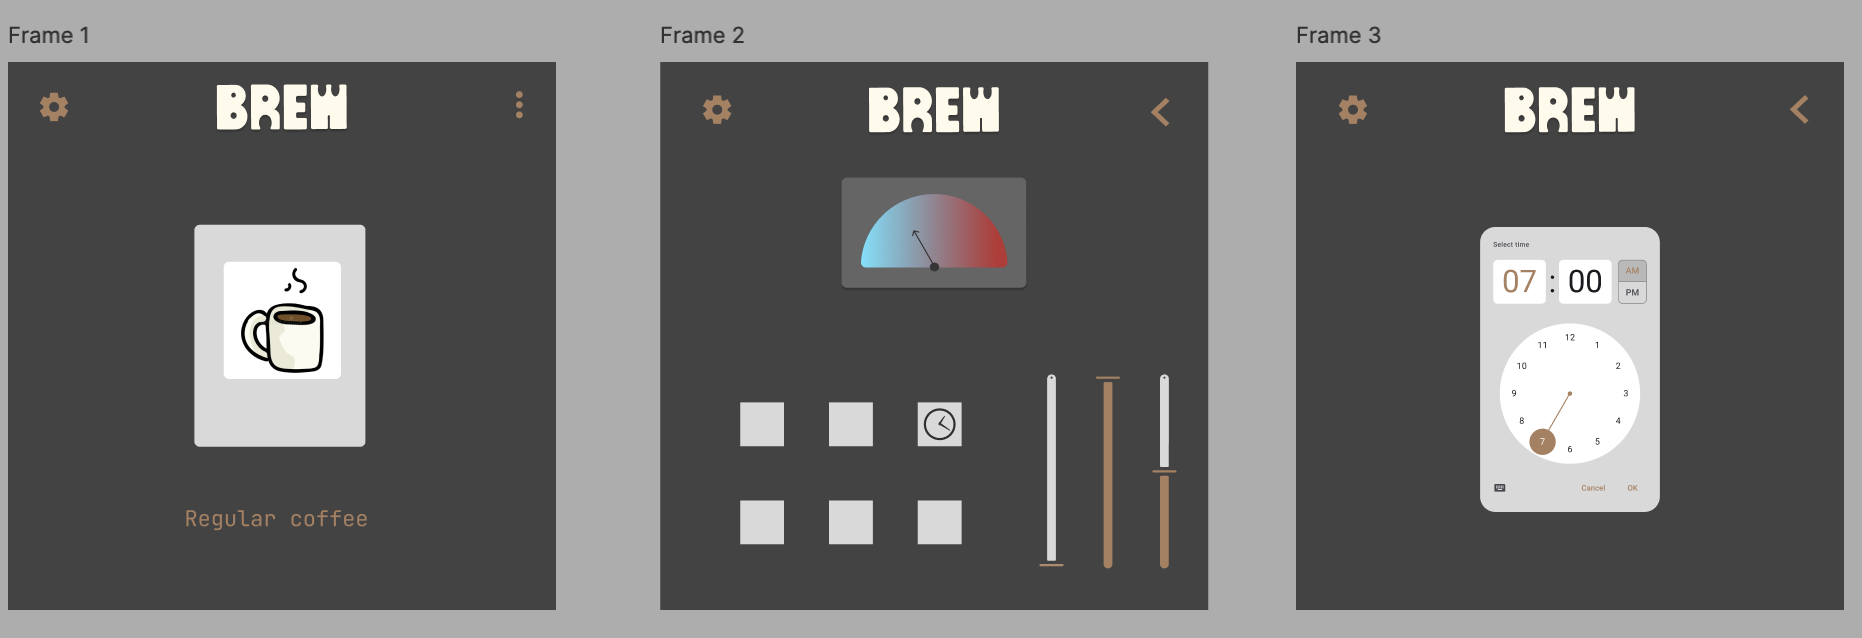
\includegraphics[width=0.8\textwidth]{bilder/sjov2.png}
    \caption{Tidig prorotyp från design studio-sessionen}
    \label{fig:tidiga3}
\end{figure}

\textbf{Designalternativ A} fokuserade på ett touchscreen-baserat gränsnit med stora kreativa grafiska representationer för information. Syftet var att skapa något tydligt som ändå hanterade avancerade inställningar väl. Detta alternativ valdes bort eftersom representationerna hade dålig överensstämmelse med mentala modellen som en typisk användare har, och var istället mer anpassat till de som redan har kunskap inom avancerat kaffe bryggning.

Exempelvis så fokuserade gränsnitet på förhålanden mellan bönor och vatten, och i termer av massa. Redan inom gruppen skappade detta förvirring, då det inte va uppenbart hur mycket man ska brygga för att få en kopp, och om det skulla göra kaffet svagare eller inte.

Det beslutades dock att id\'eerna var rimliga för ett "advanced mode" i framtida iterationer.

\textbf{Designalternativ B} erbjöd ett alternativ som använde sig av fysiska knappar och reglage. All navigation styrdes av ett hjul. Att välja alternativ var mer intuitivt, men reglagen gjorde det svårare att använda avancerade inställningarna, och var inte praktiskt för att namnge profiler. 

\textbf{Designalternativ C} fokuserade på touch, och tillämpade en “plattare” design. Fler alternativ, inställningar, och funktioner kunde visas, och färre steg var obligatoriska för att brygga kaffe. Därför valdes det att basera första digitala prototypen på detta alternativ.
\subsection{Iteration 2: Första digitala prototyp}


Baserat på feedback från lo-fi-testerna utvecklades den första digitala prototypen.  Detta gjordes genom en bedömning för varenda design mål för alla koncept samt vilka design constraints de hade. Koncepten för avancerat läge togs från alternativ A, preset design togs från alternativ B och C, och schemaläggning inspireras av fig alternativ C. Det skapades först en lofi prototyp, och utefter den skapades en interaktiv prototyp med javascript. Huvudsakliga vyer inkluderar: startsidan, sidmenyn, “manage profiles”, “schedule coffee” och "create profile".

\begin{figure}{H}
    \begin{center}
        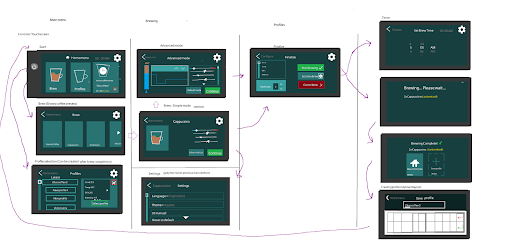
\includegraphics[width=0.95\textwidth]{bilder/victorM.png}
    \end{center}
    \caption{Merged koncept av alla gruppmedlemmars första koncept.}
    \label{fig:mergedV}
\end{figure}

\subsubsection{Startsida}

Startsidan designades för att tillåta användaren att brygga sin kaffe så fort som möjligt. Genom att flytta alla diagram och inställningar till andra delar av gränssnittet blir det tydligt vilka alternativ man har. Om man bara vill ha kaffe, då trycks det på quick brew. Om man vill leka med inställningar eller presets så trycker man på plus. Mellan lofi och hifi prototyperna så flyttades även diagrammen till “edit profile” skärmen. Tillsammans bidrar detta till teoretisk bättre visibility, samt bättre sammanhang mellan användarens mentala modell och gränssnitt. Exempelvis är det tydligt att “quick brew” inte är en preset, och kan inte förändras. 

Inom denna prototyp så var affordance i huvudfokus pågrund av idén för en kaffemaskin så skulle touchskärm integreras pågrund av constraints för fanns för fysiska knappar, men dessutom så kan det vara så att skärmen inte är tillräckligt stor, så pga visibility så var därför affordance i huvudfokus. Tydligaste exemplaret av affordance är när man ska klicka "Brew" där menyn visas i block där den längst till vänster visade att man kunde "swipea" höger. Risken med detta var dock memorability ifall man kommer ihåg att ett visst preset fanns längst till höger om man ville bara brygga en enkel kopp macchiato t.ex. Alla knappar inom menyn ska dessutom vara lätt igenkännbara med att de går att trycka på, så de mesta knappar ska ha en rektangulär form med runda kanter som påminnelse att de går att trycka på för att uppfylla design constraint affordance.

\begin{figure}[H]
    \centering
    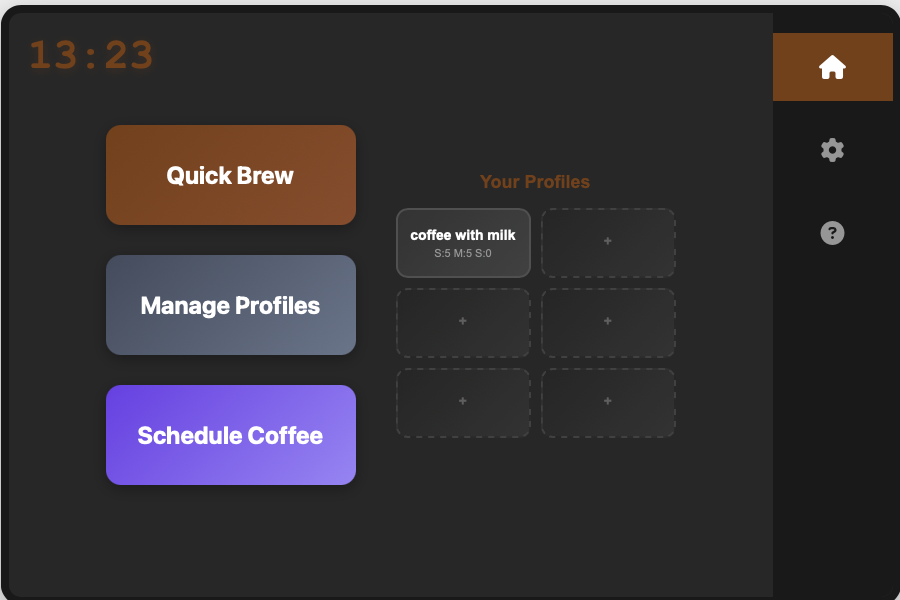
\includegraphics[width=0.6\textwidth]{bilder/start.png}
    \caption{Första versionen av startsidan}
    \label{fig:startsida_v1}
\end{figure}

Huvudelementen är:
\begin{itemize}
    \item \textbf{Quick Brew}: Placerad i toppen av menyn till vänster, för att göra det tydligt att den inte är en preset, samt är den stor så att det blir en av de första sakerna som märks av användaren. Detta minskar chansen att en användare inte lyckas brygga kaffe alls.     

    \item \textbf{Preset area}: Placerat till höger, och någorlunda mindre än menyn till vänster. Strukturen görs så att mindre scrollning behövs jämfört med tidiga prototyper, och skapar en tydlig skillnad mellan det man kan ändra, och det som är permanent. 
\end{itemize}

\subsubsection{Manage Profiles}

Sidan designades för att tillåta användaren att redigera eller ta bort profiler. Elementen ordnas i en enkel lista för att göra det så tydligt som möjligt för användaren att de redigerar och inte brygger. Valet att ha en separat skärm för detta gjordes för att förenkla startsidan så mycket som möjligt.
\begin{figure}[H]
    \centering
    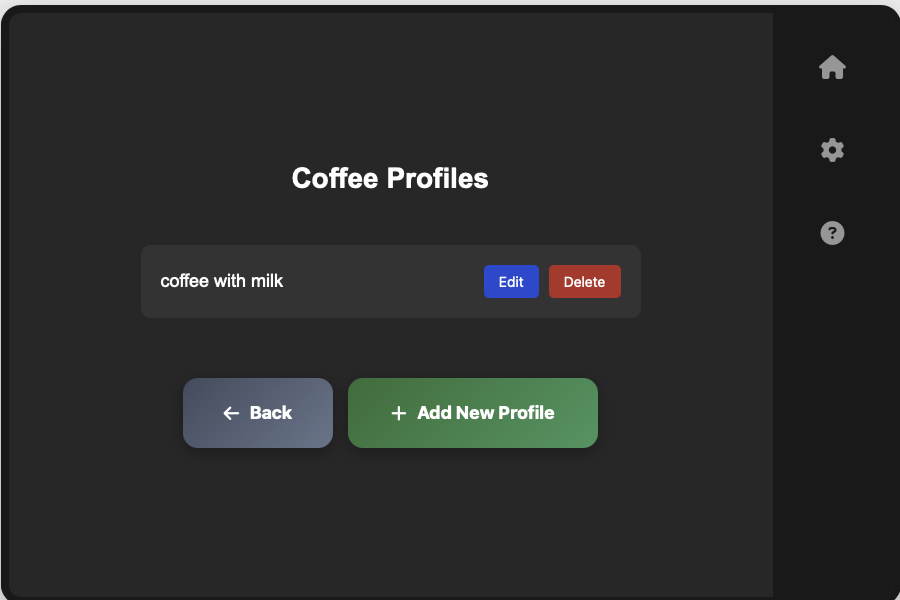
\includegraphics[width=0.6\textwidth]{bilder/manage.png}
    \caption{Första versionen av "manage profles" sidan}
    \label{fig:manage_v1}
\end{figure}

\subsubsection{Schedule Coffee}

Sidan designades för att tillåta användaren att schemalägga en bryggning. Layouten följer samma format som “Manag Profiles"-sidan. Genom att göra det konsekvent förstår användaren åter att listan finns för att redigera, och att knapparna är permanenta. 
\begin{figure}[H]
    \centering
    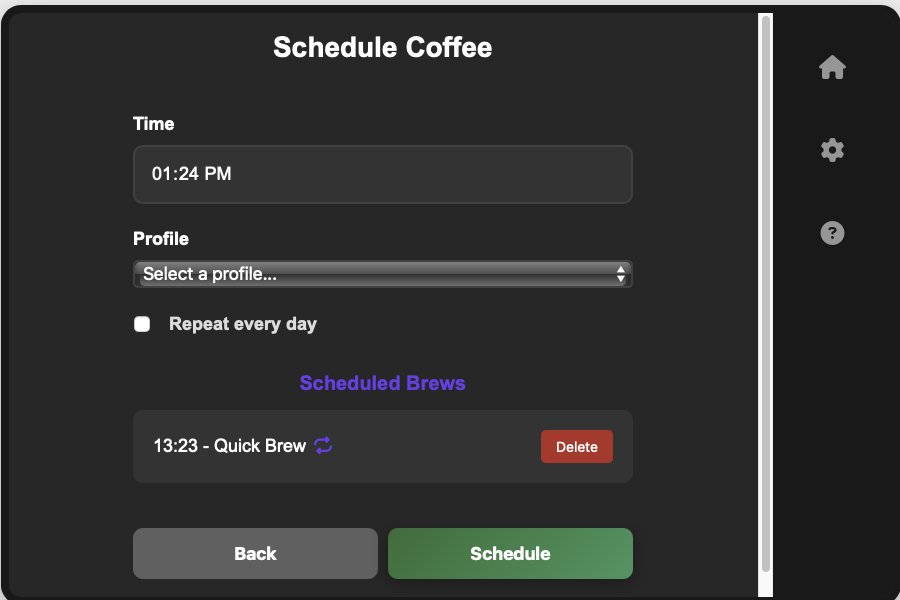
\includegraphics[width=0.6\textwidth]{bilder/schedule.png}
    \caption{Första versionen av "schedule coffee" sidan}
    \label{fig:schedule_v1}
\end{figure}

Huvudelementen är:
\begin{itemize}
    \item \textbf{Scheduled Brews}: Följer samma principer som "manage profiles".
    \item \textbf{Select a profile}: Använder sig av en "pop down menu" för att minska hur mycket information behövs bearbeta direkt då en användare får upp skärmen. 
    \item \textbf{Time}: Placerat längst upp, eftersom det är det användaren tänker på först när de vill schemalägga något. 
\end{itemize}


% ================ Create Profile ==================
\subsubsection{Create Profile}
Det bestämdes tidigt att “Create pofile” sidan var väldigt viktig. Den behöver vara enkel nog för att inte skrämma bort användare som inte har stor kompetens inom kaffe-bryggning eller teknik, men också vara intuitiv, effektiv, och kul att använda för de som har dem kompetenserna. 

\begin{figure}[H]
    \centering
    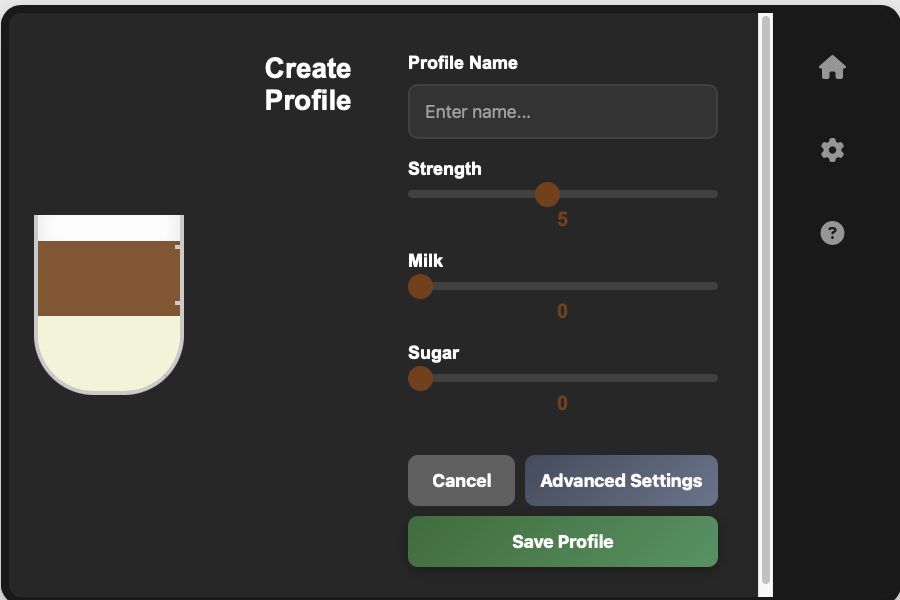
\includegraphics[width=0.6\textwidth]{bilder/brew.png}
    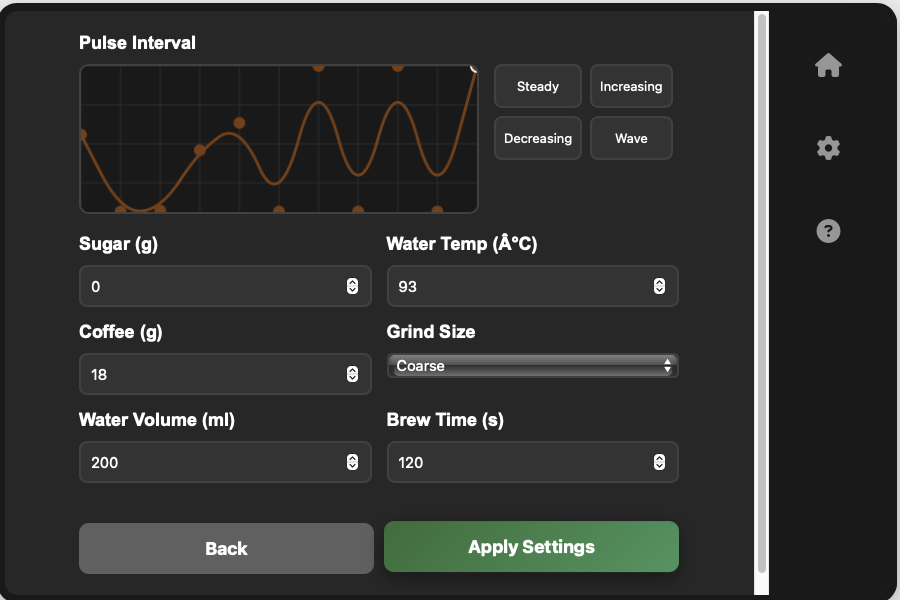
\includegraphics[width=0.6\textwidth]{bilder/advancedshit.png}
    \caption{Första versionen av "create profiles" sidan}
    \label{fig:create_v1}
\end{figure}
\textbf{Utility}: Prototypen utnyttjar verktyg för att kunna utföra kaffebryggning på både ett enkelt och avancerat sätt, men på en funktionalitet så att användaren får specificera hur i detalj de vill gå. Användaren borde kunna ändra enkla saker som förekommer oftast vid kaffebryggning, såsom mjölk, styrka och socker, då det är en väldigt vanlig smaksak. När det dock kommer de som vill experimentera lite mer med sitt kaffe så finns därför ett avanced mode för att kunna vara så precis som möjligt med sin kaffebryggning. Där kan användaren konfigurera pulsintervall för kaffebryggning, andel socker i gram, temperaturen på kaffet, andel kaffe i gram, texturen på kaffet, andel vatten som används och hur länge det ska bryggas i.

\textbf{Effectiveness}: Eftersom att den ordinära användaren inte vill trycka in andel socker eller vattentemperatur så borde de inte finnas inom defaultkonfigurationen pågrund av att en kaffemaskin främst ska göra kaffe på ett snabbt och effektivt sätt, så om man behöver knappa in mer saker i en defaultkonfiguration för kaffe så kan det göra användaren överväldigad med andelen funktioner för att bara brygga kaffet. Därför finns advanced mode som en separat meny för de som är medvetna om att de kan lite mer om kaffe men samtidigt ska det inte låsa ut användare för att pröva och experimenta med sitt kaffe om de vill.

\textbf{Efficiency}: Profilmenyn är designat så att vid defaultkonfigurationen av att skapa en profil så är det simplicietet som är i prioritet, så att användaren kan brygga kaffe så snabbt som möjligt med ett enkelt utseende på skärmen. Om användaren vill gå in i detalj så finns advanced mode för det alternativet. Det är medvetet att det kommer ta mer tid, men samtidigt så går det ändå att göra menyn tilräckligt enkel för att inte skrämma bort användare som vill testa sig fram genom menyerna. Detta görs t.ex genom presets för pulsintervallet.

\textbf{Learnability}: Med ett enkelt gränssnitt så ska det vara enkelt att göra sitt kaffe men inte "skrämma" användare för att experimentera med advanced modes funktioner. Därför behövde vara enkel att lära sig med att inte ha för många funktioner med samtidigt tillfredsställa de som vill konfigurera sitt kaffe.

Advanced menyn förenklades med att tydliggöra pulsintervallet, samt ge användaren presets att välja från, för att hen ska kunna få en känsla för gränssnittet.


% ================  Side menu ==================
\subsubsection{Sidmenyn}
Sidmenyn designades för att ge snabb åtkomst till viktiga funktioner som kan behövas oavsett var man är i gränssnittet.  

Huvudelementen är:
\begin{itemize}
    \item \textbf{Hem Knappen}: Placerad längst upp för att skapa ett sätt för användaren att alltid kunna komma tillbaka till startsidan. Detta hjälper mycket med att minska antalet fel som inte går att åtgärda. 
    \item \textbf{Inställningar och hjälp}: Synligt placerad eftersom användaren ska alltid kunna få hjälp. Kravet för användaren att behöva komma ihåg saker minskas.
\end{itemize}



% ========================= CONTINUING HERE ======================

\subsection{Iteration 3}

Efter användbarhetstester i iteration 2 identifierades flera problem (se avsnitt \ref{sec:resultat_test}). Följande ändringar gjordes:


\begin{figure}[H]
    \centering
    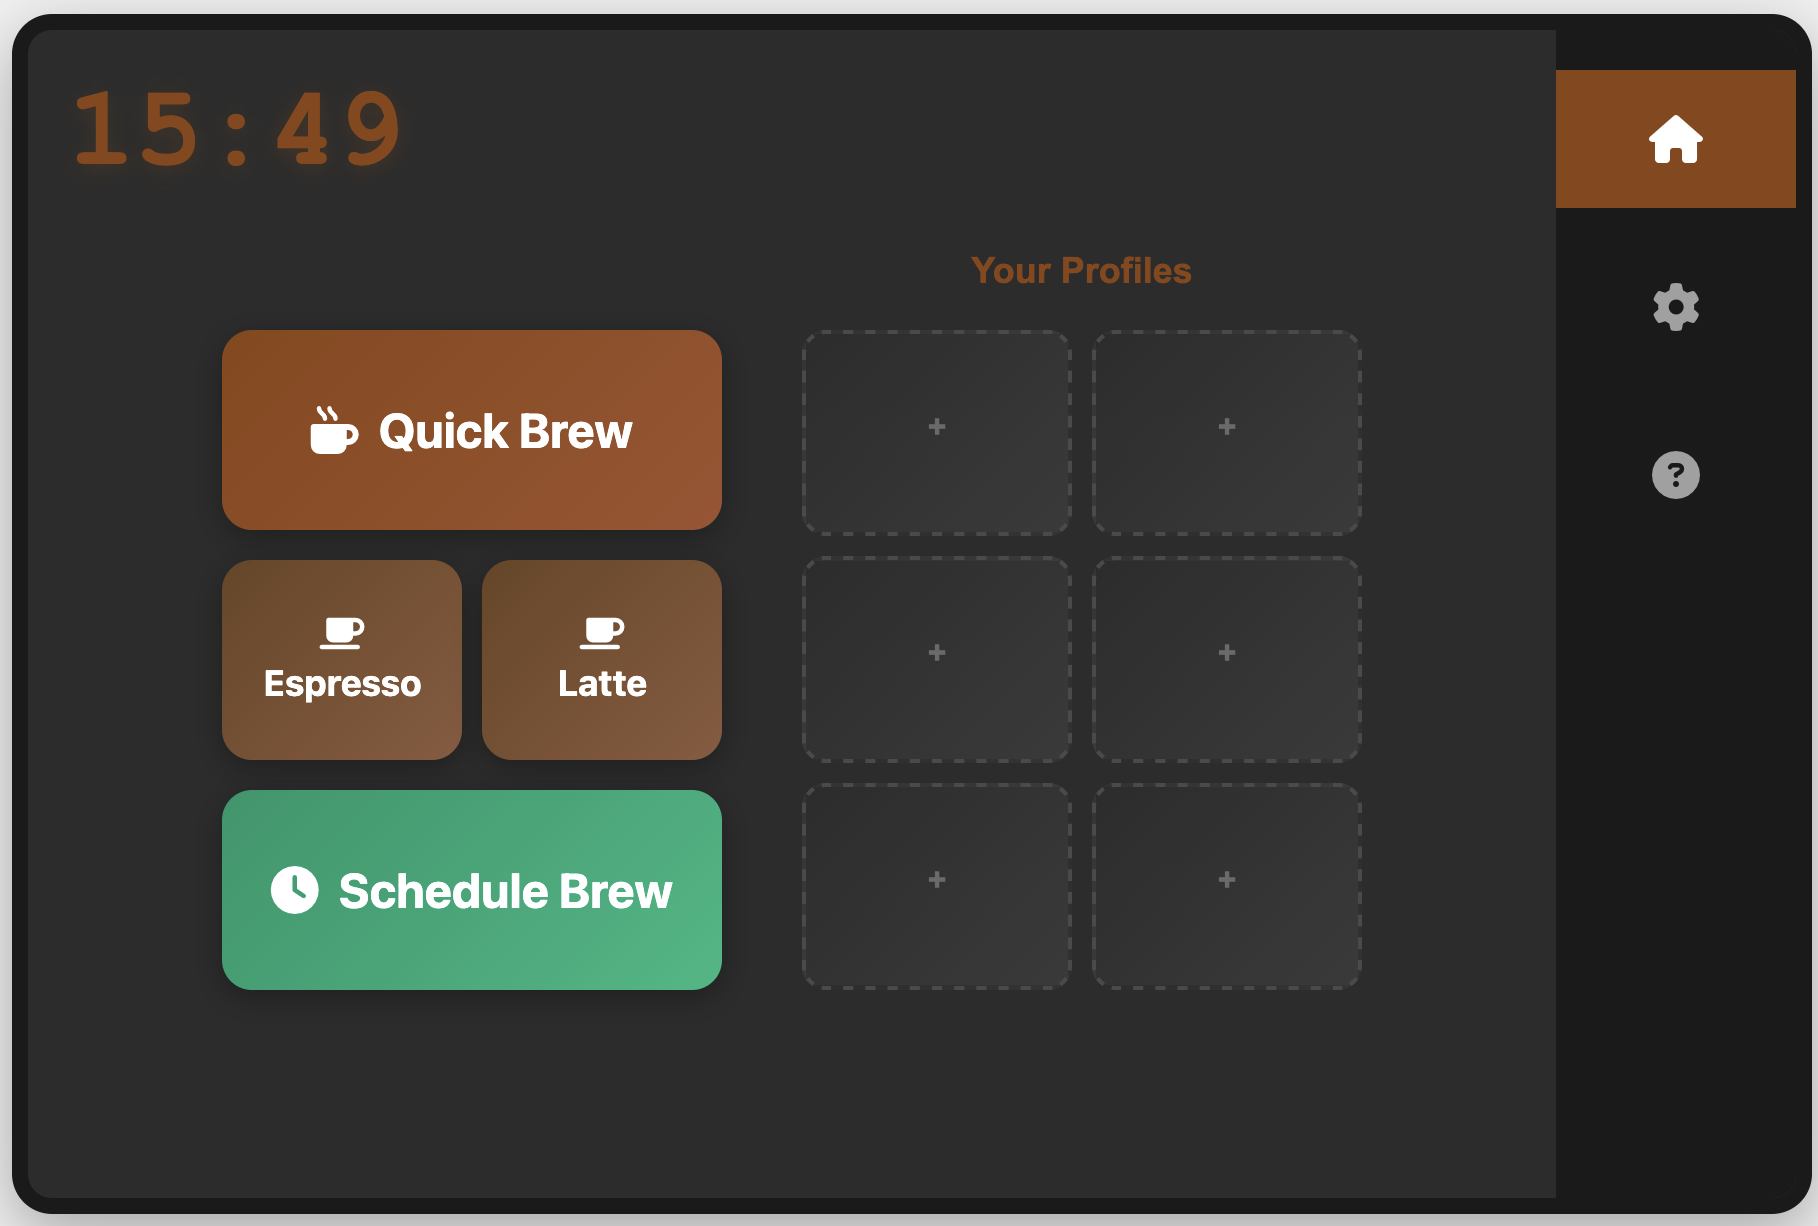
\includegraphics[width=0.6\textwidth]{bilder/3problem1-25.png}
    \caption{ förändringar som gjorts för att lösa problem 1, 2 och 5}
    \label{fig:forbattring1}
\end{figure}

\textbf{Problem 1:} Användare hade svårt att identifiera vad knappar gjorde direkt, och tyckte att det var krävande att behöva läsa så mycket text.  

\textbf{Lösning:} Fler ikoner lags till som anseddes förbättra tydligheten av knapparna samt följer det Nielsens (citation) design heurestic “Recognition over recall”. 

\textbf{Problem 2} Flera användare tyckte att det borde finnas färdiga profiler 

 \textbf{Lösning:} Färdiga profiler skapades. De går att använda profilerna som avgångspunkter för att skapa eget recept, detta tycktes göra processen enklare för de som inte har mycket erfarenhet inom kaffe.  

 \textbf{Problem 3} Vi fick feedback att färgerna var ibland inte konsekventa, och att de var ibland otydliga.  

\begin{figure}[H]
    \centering
    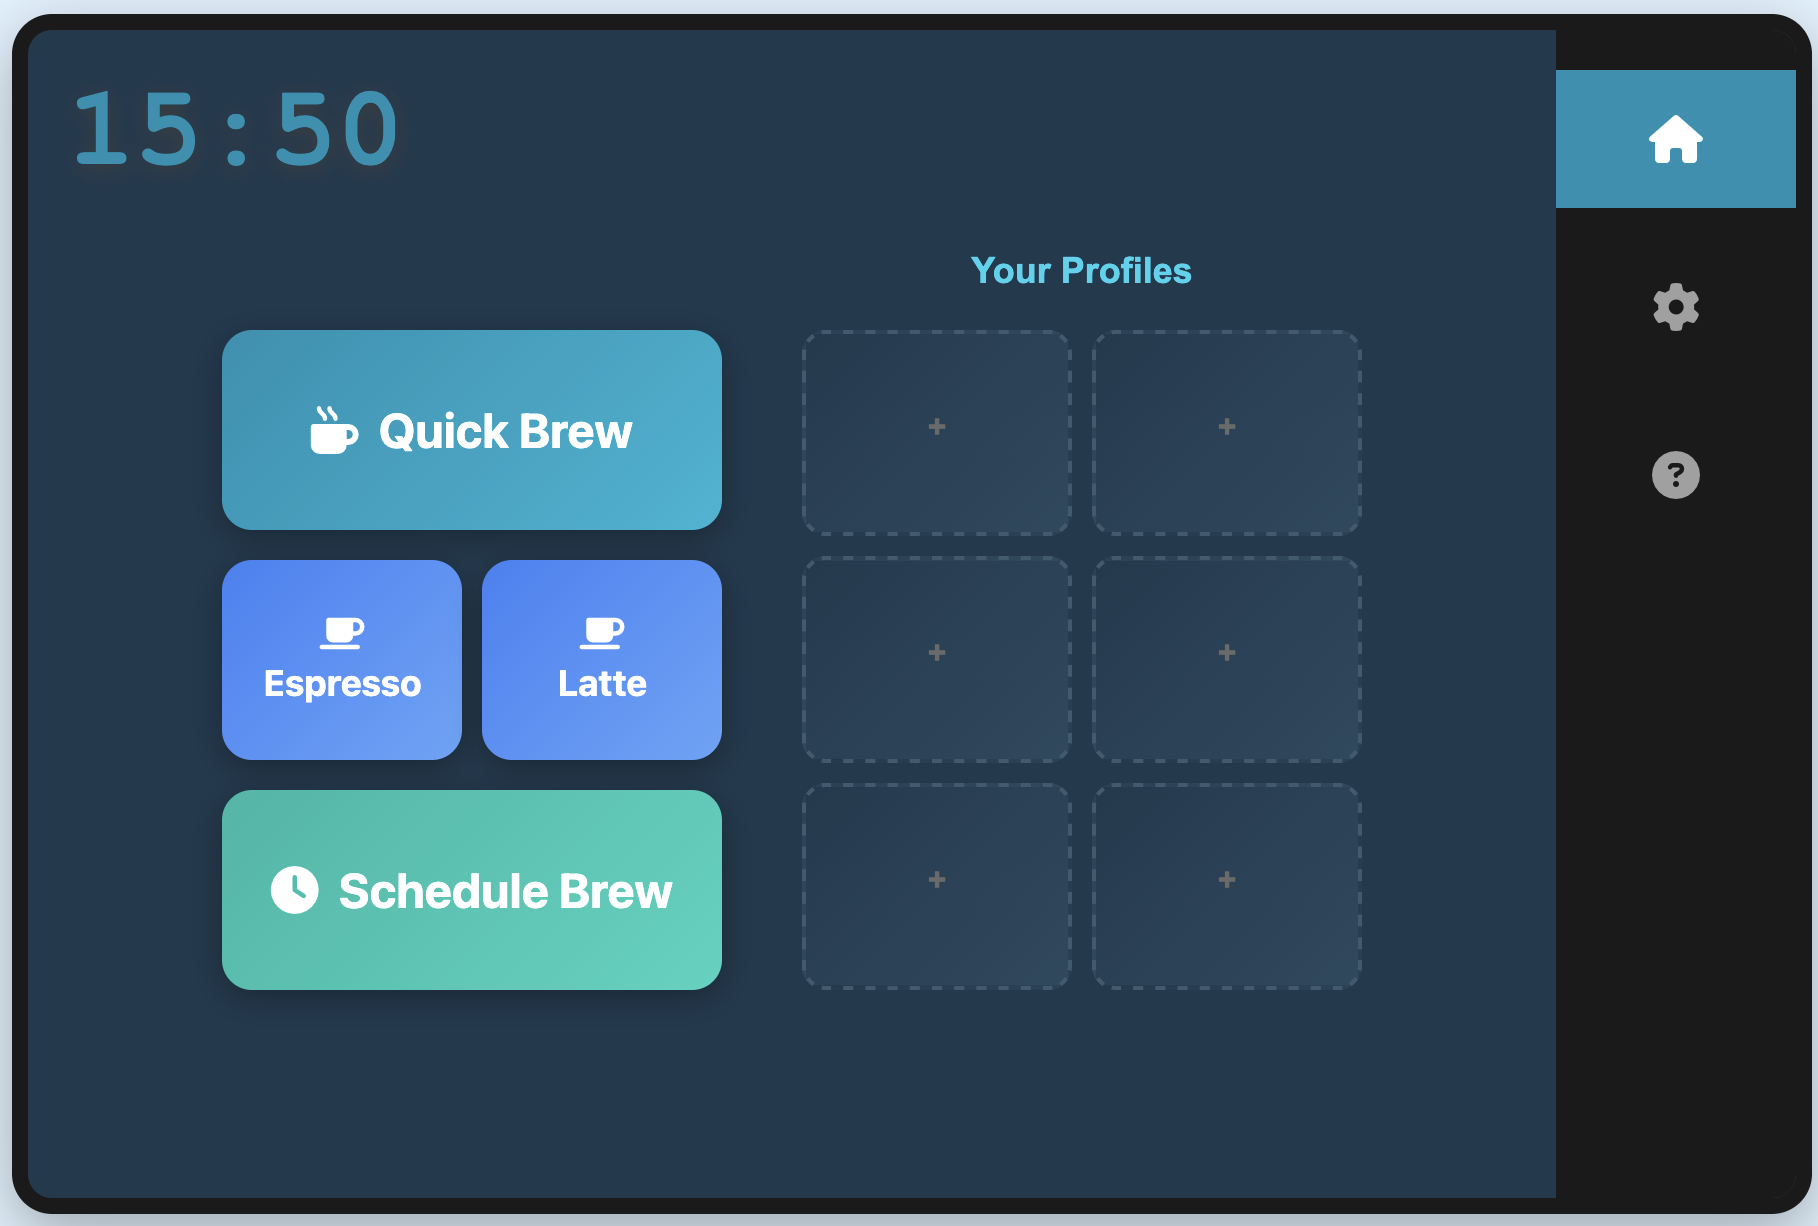
\includegraphics[width=0.6\textwidth]{bilder/3problem2.png}
    \caption{ förändringar som gjorts för att lösa problem 3}
    \label{fig:2forbattring2}
\end{figure}
\textbf{Lösning:}  flera påpekade detta problem, men hade inte specifika krav eller exempel. På grund av detta samt att flera andra ville ha valbara färgtema, så var det naturligt att implementera några färgteman.   

\textbf{Problem 4} Gränssnittet för att schemalägga bryggning hade fåt lite kritik över des icke intuitive design. 

\begin{figure}[H]
    \centering
    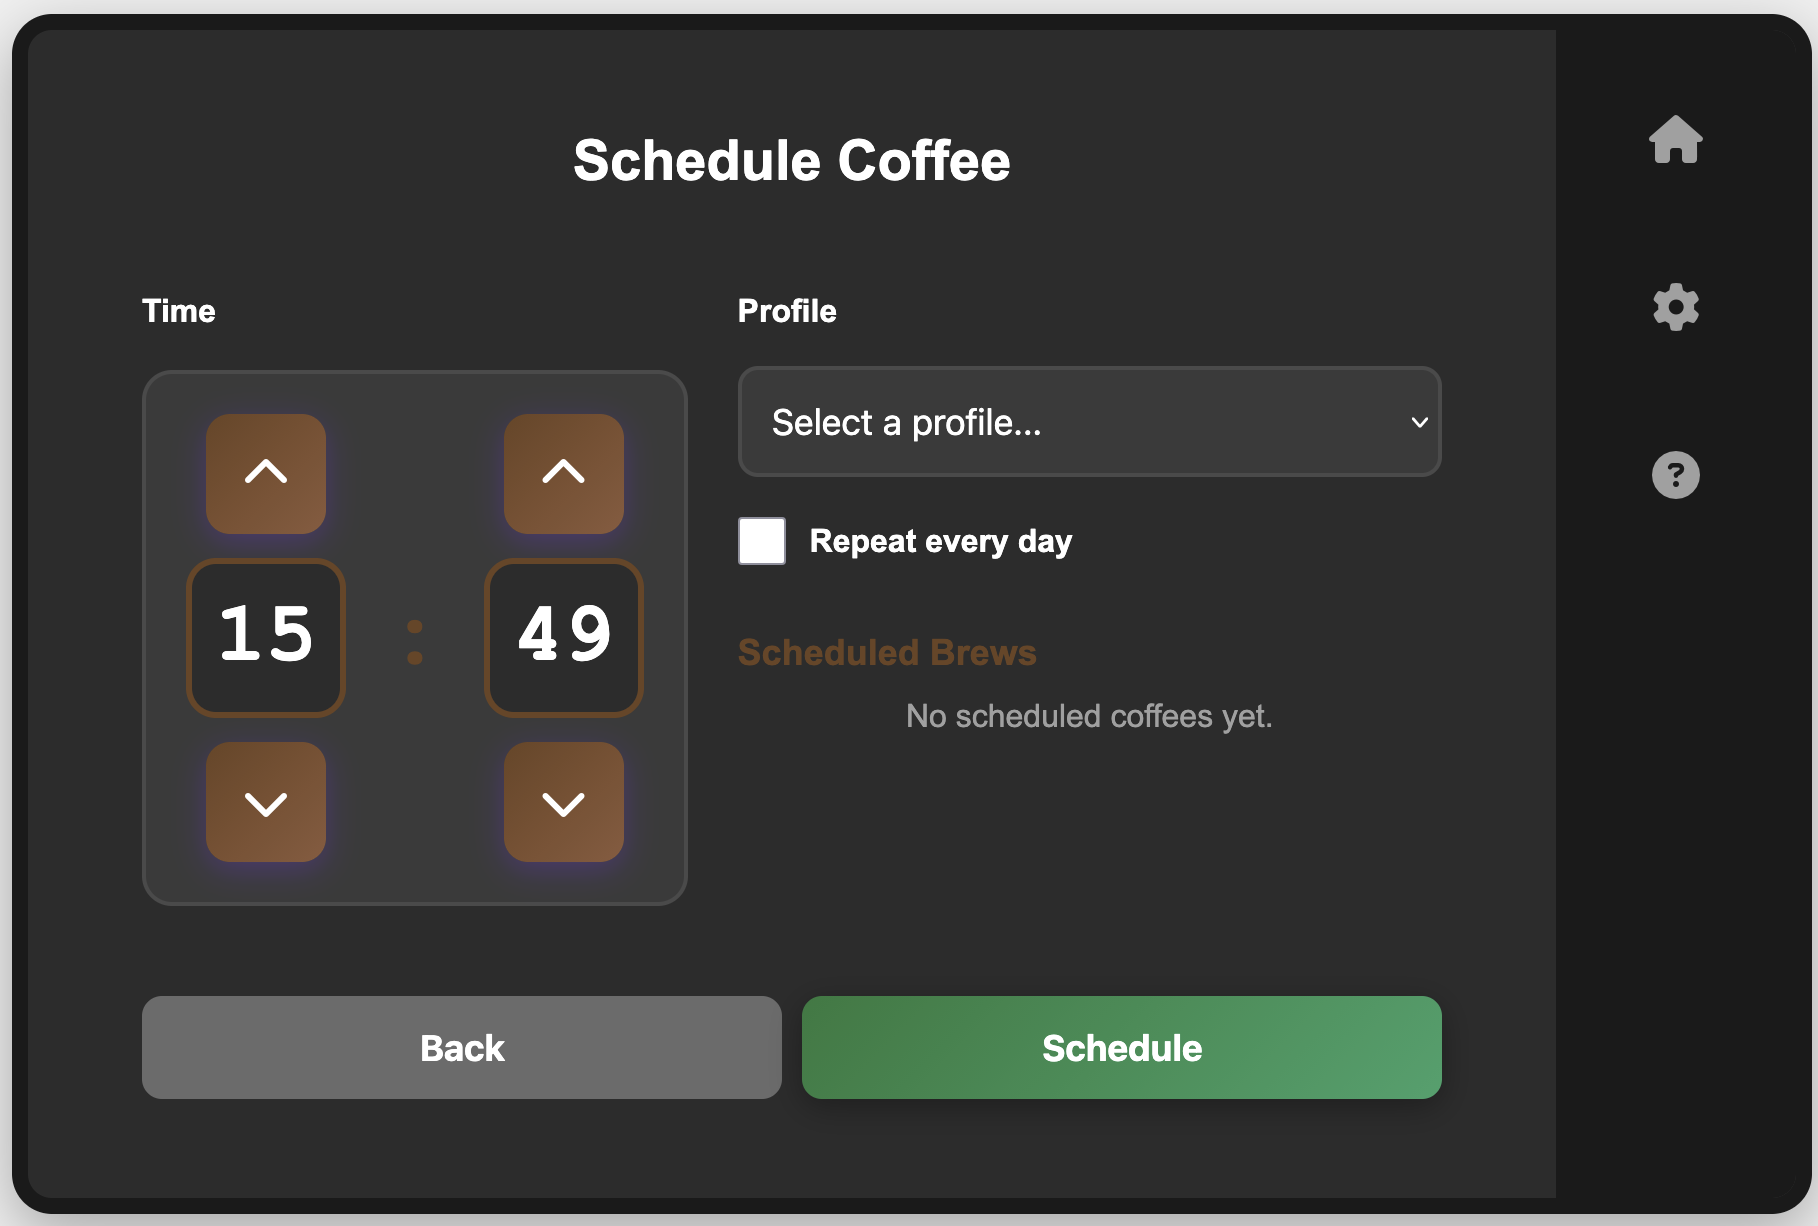
\includegraphics[width=0.6\textwidth]{bilder/3problem4.png}
    \caption{ förändringar som gjorts för att lösa problem 4}
    \label{fig:forbattring3}
\end{figure}
\textbf{Lösning} Det gjordes om så att knappar användes för att välja tid. Detta anseddes vara lättare än att skriva in tiden med ett touch tangentbord på skärmen  

 \textbf{Problem 5} “Profile manager” sidan förvirrade visa användare.  

\textbf{Lösning:} Detta var ganska logiskt, eftersom det går att skapa profiler från startsidan så borde det också gå att redigera dem där. Därför lags det till en “edit” knapp  på var profil i startsidan, och delete knappen flytades in i “edit profile” vyn.  Därefter så togs bort “Profile manager” sidan.  






\subsection{Iteration 4}

Efter användbarhetstester i iteration 3 identifierades flera problem (se avsnitt \ref{sec:resultat_test}). Följande ändringar gjordes:

\textbf{Problem 1:} Kontrasten gjorde viss text otydlig eller svår att läsa.  

  

\textbf{Lösning:} Det lags till en lysande effekt till text där det anseddes vara ett problem med kontrast. Samt lags det till en “blinking” effekt till visa textfält för att förtyda att de var obligitoriska.  

  
\begin{figure}[H]
    \centering
    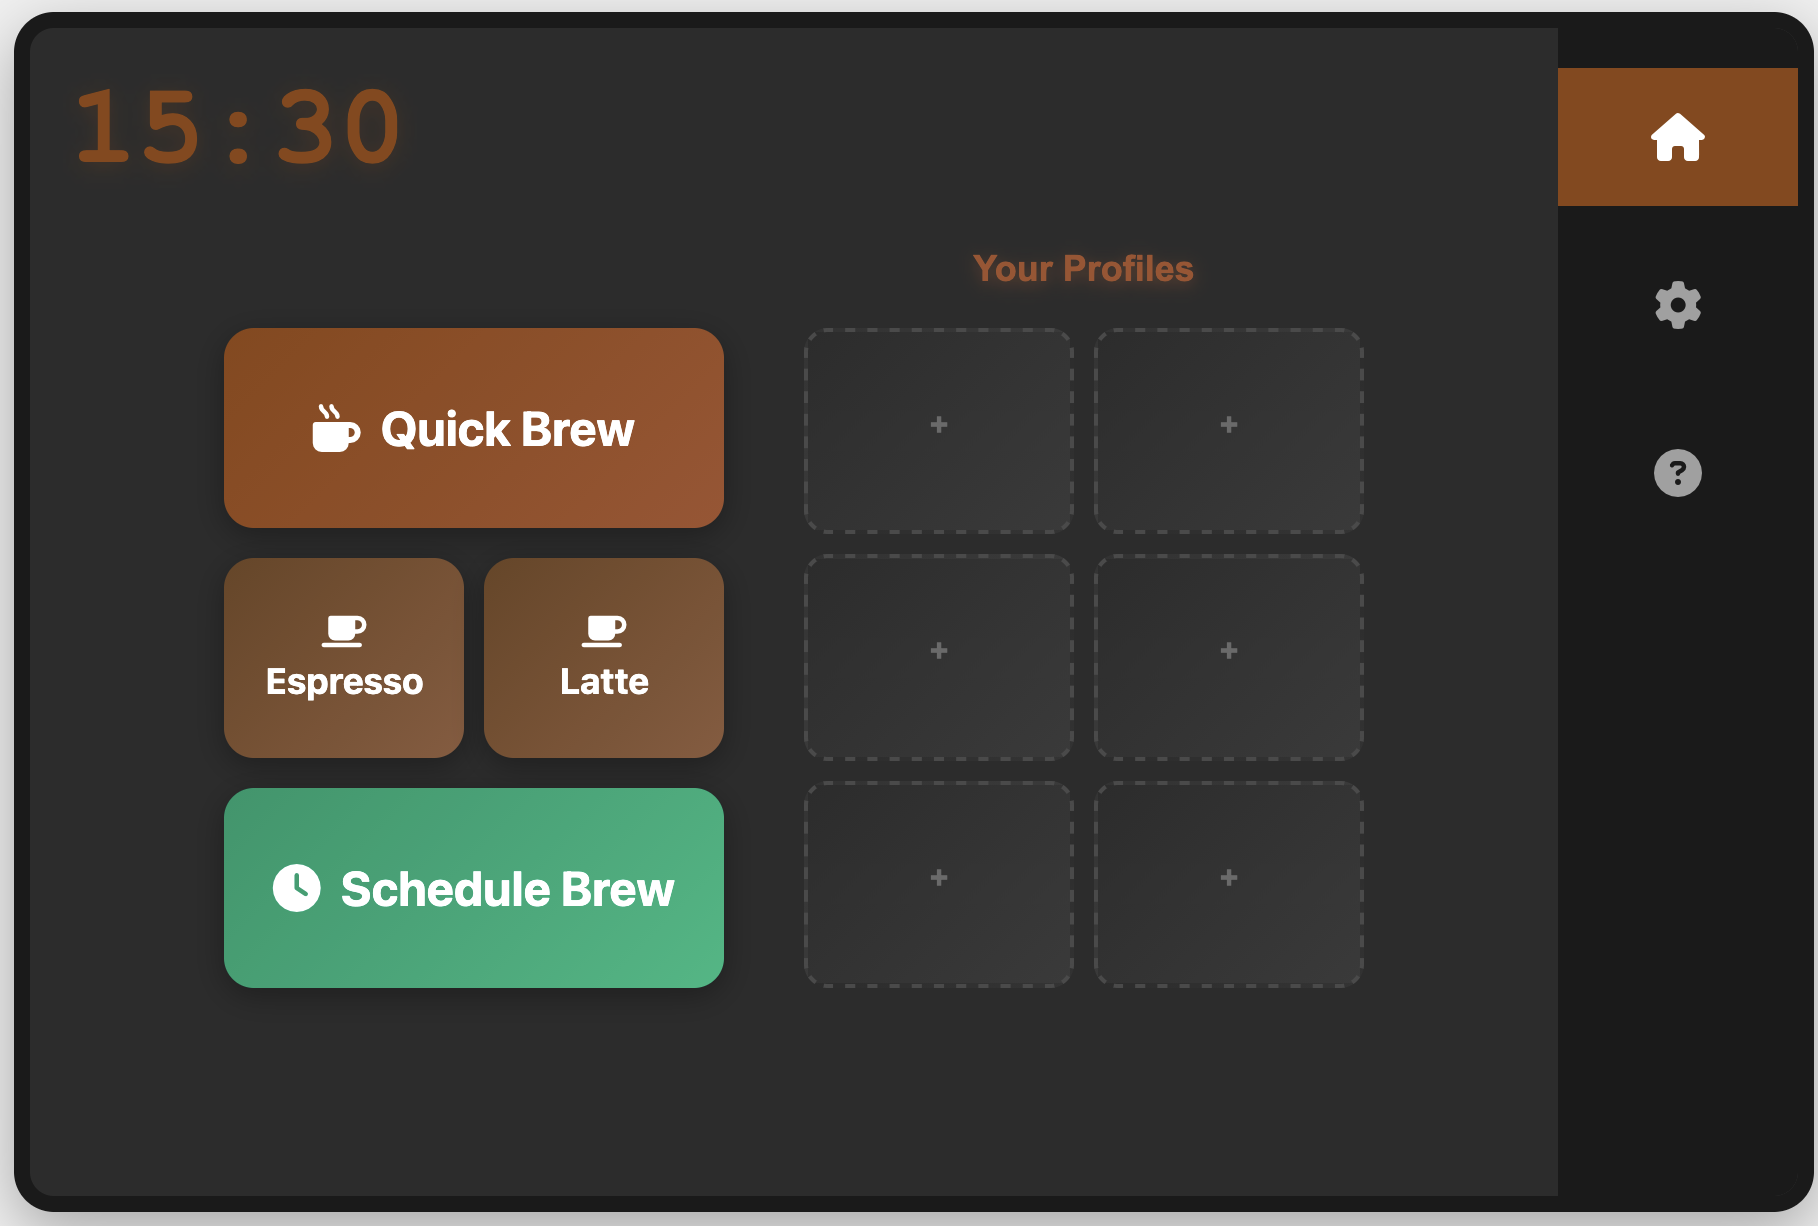
\includegraphics[width=0.6\textwidth]{bilder/3problem1.png}
    \caption{ förändringar som gjorts för att lösa problem 1}
    \label{fig:forbattring4}
\end{figure}

\textbf{Problem 2} “Confirm” menyer var ej konsekventa och ibland saknades det en “cancel knapp” 

  

\textbf{Lösning:} En “cancel” knapp lags till i varje “confirm” meny, samt  
standardiserades de över hela gränssnittet.  

\textbf{Lösning:}  

Detta var ganska logiskt, eftersom det går att skapa profiler från startsidan så borde det också gå att redigera dem där. Därför lags det till en “edit” knapp  på var profil i startsidan, och delete knappen flytades in i “edit profile” vyn.  Därefter så togs bort “Profile manager” sidan.  


\begin{figure}[H]
    \centering
    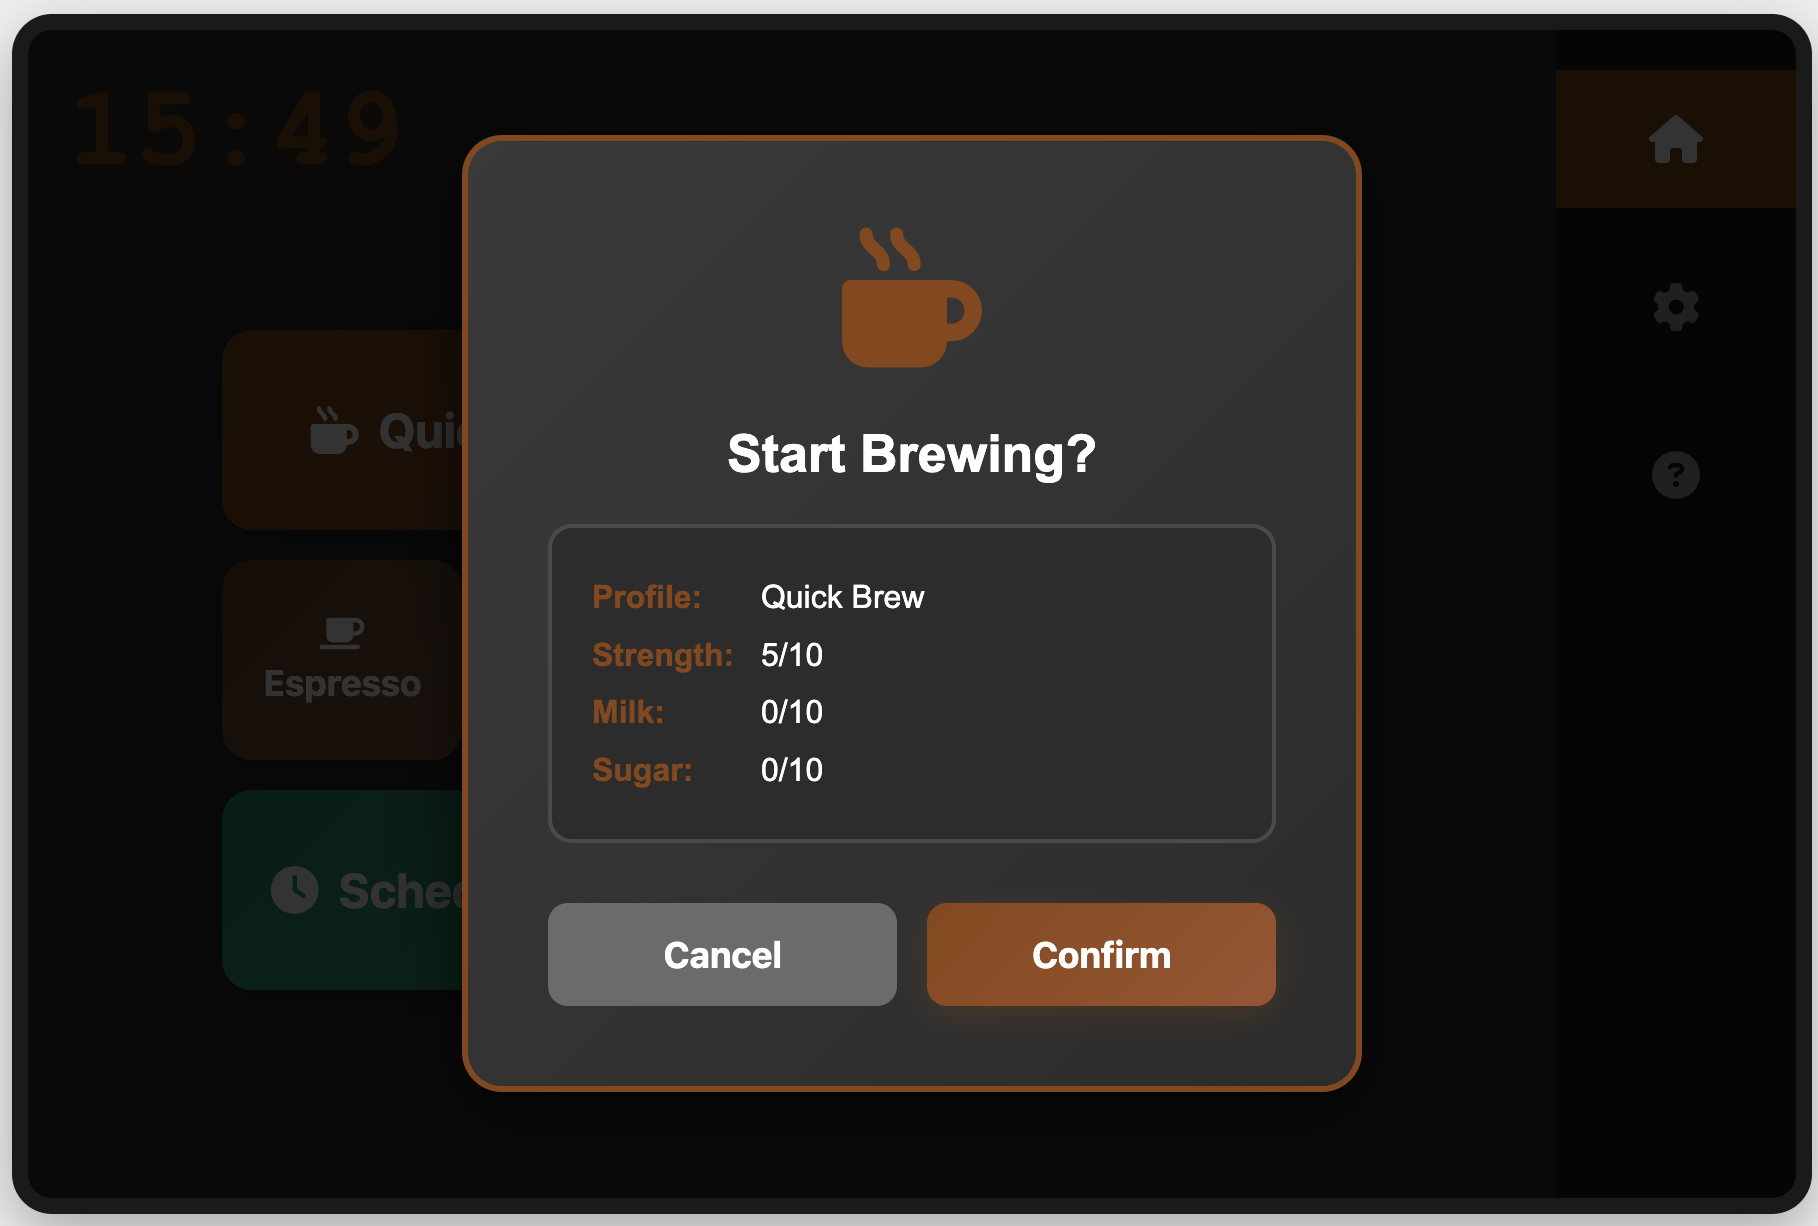
\includegraphics[width=0.6\textwidth]{bilder/4problem2.png}
    \caption{ förändringar som gjorts för att lösa problem 2}
    \label{fig:forbattring5}
\end{figure}


\subsection{Slutgiltig design}

\textit{[Presentera den slutgiltiga designen]}

Den slutgiltiga designen är resultat av [antal] iterationer och integrerar feedback från [antal] användare. Fullständiga vyer finns i Bilaga C.

Huvudsakliga designprinciper som tillämpats:
\begin{itemize}
    \item \textbf{Konsistens}: Alla vyer följer samma layoutmönster...
    \item \textbf{Feedback}: Användaren får tydlig återkoppling när...
    \item \textbf{Affordance}: Interaktiva element signalerar tydligt...
\end{itemize}




\subsection{Designbeslut och motiveringar}

\textit{[Sammanfatta viktiga designbeslut]}

\begin{table}[h]
\centering
\begin{tabular}{|p{4cm}|p{5cm}|p{4cm}|}
\hline
\textbf{Designbeslut} & \textbf{Motivering} & \textbf{Teoretisk grund} \\
\hline
Navigation i top bar & Användarna förväntar sig... & Mental modeller \cite{sharp2019} \\
\hline
Färgschema: ... & Tillgänglighet och kontrast & WCAG-riktlinjer \\
\hline
... & ... & ... \\
\hline
\end{tabular}
\caption{Sammanställning av huvudsakliga designbeslut}
\end{table}

\newpage

\section{Resultat}
\label{sec:resultat_test}

\subsection{Resultat från jämförelser med befintliga lösningar}

\textit{just do comparisons and some krav/ goals based on them...}


\subsubsection{Identifierade teman}

Genom tematisk analys identifierades följande huvudteman:

\textbf{Tema 1: [Temats namn]}

[Antal] av deltagarna nämnde problem relaterade till [beskriv]. En deltagare uttryckte: \textit{"[citat]"}. Liknande upplevelser rapporterades av...

\textbf{Tema 2: [Temats namn]}

[Fortsätt beskriva teman objektivt]


\subsubsection{Identifierade behov}

Baserat på intervjudata identifierades följande användarbehov:
\begin{itemize}
    \item Behov 1: [Beskriv]
    \item Behov 2: [Beskriv]
    \item ...
\end{itemize}


\subsection{Resultat från användbarhetstester - Iteration 2}

Femton användare deltog i användbarhetstester av prototyp version 2. Varje deltagare fick genomföra 4 uppgifter, men enkäten hade inte frågar om fjärde uppgiften. 

\subsubsection{Information om deltagare}

\begin{table}[H]
\centering
\begin{tabular}{|l|c|}
\hline
\textbf{Ålder} & \textbf{Antal} \\
\hline
20s:  & 4  \\ 
50s:  & 4  \\
80s:  & 1  \\
\hline
\end{tabular}
\caption{Ålder bland deltagare}
\label{tab:age1}
\end{table}

\begin{table}[H]
\centering
\begin{tabular}{|l|c|}
\hline
\textbf{Ålder} & \textbf{Antal} \\
\hline
nej  & 4   \\
ja  & 5  \\
\hline
\end{tabular}
\caption{Deltagare som använt en liknande produkt}
\label{tab:exp1}
\end{table}



\subsubsection{Kvantitativa resultat}

\textbf{Genomförandetid}

Tabell \ref{tab:tid2} visar tid för att genomföra varje uppgift.

\begin{table}[h]
\centering
\begin{tabular}{|l|c|c|c|}
\hline
\textbf{Uppgift} & \textbf{Medeltid (s)} & \textbf{Min (s)} & \textbf{Max (s)} \\
\hline
Uppgift 1:  & 4 & 1 & 12 \\
Uppgift 2:  & 24 & 4 & 60\\
Uppgift 3:  & 23 & 1 & 60\\
\hline
\end{tabular}
\caption{Tid för genomförande av uppgifter}
\label{tab:tid2}
\end{table}

\textbf{Framgångsgrad}

Figur \ref{fig:success_rate} visar hur många deltagare som lyckades genomföra varje uppgift utan hjälp.

\begin{figure}[ht]
    \centering
    % \includegraphics[width=0.7\textwidth]{bilder/success_rate.png}
    \caption{Framgångsgrad för varje uppgift (antal användare som klarade uppgiften utan hjälp)}
    \label{fig:success_rate}
\end{figure}

\textbf{Identifierade problem}

Totalt identifierades 20 unika användbarhetsproblem. Tabell \ref{tab:problem} sammanfattar de mest förekommande problemen.
\begin{table}[h]
\centering
\begin{tabular}{|p{6cm}|c|c|}
\hline
\textbf{Problem} & \textbf{Antal som drabbades} & \textbf{Allvarlighetsgrad} \\
\hline
Problem 1: Colors misleading or hard to look at & 6/15 & Medel\\
Problem 2: Time scheduling difficult & 2/15 &  Låg \\
Problem 3: Getting to edit profile unintuitive & 6/12 & Hög\\
\hline
\end{tabular}
\caption{Identifierade användbarhetsproblem och deras allvarlighetsgrad}
\label{tab:problem}
\end{table}


\subsubsection{Kvalitativa resultat}

Under testerna observerades följande beteenden:

\textbf{Navigation:} Flera användare (6/15) uttryckte förvirring när de skulle redigera en profil, det var många som råkade börja brygga kaffe när de försökte redigera.

\textbf{Navigation:} 3 användare noterade att knapparna var förivrande, och att de skulle uppskattat mer symboler. 

\textbf{Färger} 6 användare klagade att färgerna var inte konsekventa eller hade problem med kontrasten. 


\subsubsection{Subjektiv tillfredsställelse}

Efter testerna fick deltagarna svara på hur svåra de tyckte var uppgift var att genomföra. Medelvärdet var 68 av 70.

% we didnt do this sus point thing... update method, also where we got these scores from.


% =========================================== WORKING ON THIS ===============================================

\subsection{Resultat från användbarhetstester - Iteration 3}

Femton användare deltog i användbarhetstester av prototyp version 3. Varje deltagare fick genomföra 5 uppgifter. 

\subsubsection{Information om deltagare}

\begin{table}[H]
\centering
\begin{tabular}{|l|c|}
\hline
\textbf{Ålder} & \textbf{Antal} \\
\hline
20s:  & 4  \\ 
50s:  & 4  \\
80s:  & 1  \\
\hline
\end{tabular}
\caption{Ålder bland deltagare}
\label{tab:age2}
\end{table}

\begin{table}[H]
\centering
\begin{tabular}{|l|c|}
\hline
\textbf{Ålder} & \textbf{Antal} \\
\hline
nej  & 4   \\
ja  & 5  \\
\hline
\end{tabular}
\caption{Deltagare som använt en liknande produkt}
\label{tab:exp2}
\end{table}

\subsubsection{Kvantitativa resultat}

\textbf{Genomförandetid}
Tabell \ref{tab:tid} visar tid för att genomföra varje uppgift.
\begin{table}[H]
\centering
\begin{tabular}{|l|c|c|c|}
\hline
\textbf{Uppgift} & \textbf{Medeltid (s)} & \textbf{Min (s)} & \textbf{Max (s)} \\
\hline
Uppgift 1:  & 3 & 1 & 14 \\
Uppgift 2:  & 14 & 6 & 51\\
Uppgift 3:  & 11 & 4 & 32\\
Uppgift 4:  & 13 & 3 & 42\\
Uppgift 5:  & 8 & 6.5 & 20\\
\hline
\end{tabular}
\caption{Tid för genomförande av uppgifter}
\label{tab:tid}
\end{table}

\textbf{Framgångsgrad}

Figur \ref{fig:success_rate2} visar hur många deltagare som lyckades genomföra varje uppgift utan hjälp.

\begin{figure}[ht]
    \centering
    % \includegraphics[width=0.7\textwidth]{bilder/success_rate.png}
    \caption{Framgångsgrad för varje uppgift (antal användare som klarade uppgiften utan hjälp)}
    \label{fig:success_rate2}
\end{figure}

\textbf{Identifierade problem}

Totalt identifierades 7 unika användbarhetsproblem. Tabell \ref{tab:problem} sammanfattar de mest förekommande problemen.
\begin{table}[H]
\centering
\begin{tabular}{|p{6cm}|c|c|}
\hline
\textbf{Problem} & \textbf{Antal som drabbades} & \textbf{Allvarlighetsgrad} \\
\hline
Problem 1: "Advanced" inställning behövs struktureras & 3/9 & Medel\\
Problem 2: Contrast mellan text och backgrund & 2/9 &  Medel \\
\hline
\end{tabular}
\caption{Identifierade användbarhetsproblem och deras allvarlighetsgrad}
\label{tab:problem2}
\end{table}


\subsubsection{Kvalitativa resultat}

Under testerna observerades följande beteenden:

\textbf{Metod} Flera användare blev förvirad av att testa ett touch gränssnitt på en dator. 

\subsubsection{Subjektiv tillfredsställelse}

Efter testerna fick deltagarna svara på hur svåra de tyckte var uppgift var att genomföra. Medelvärdet var 68 av 70.


\subsection{Jämförelse mellan iterationer}
\textbf{Jämförelse med iteration 2:}

\begin{itemize}
    \item Medeltid för uppgift 1 minskade från XX s till YY s
    \item Framgångsgrad för uppgift 2 ökade från XX\% till YY\%
    \item Antal identifierade problem minskade från X till Y
\end{itemize}

Figur \ref{fig:comparison} visar jämförelse mellan iterationerna.

\begin{figure}[ht]
    \centering
    % \includegraphics[width=0.8\textwidth]{bilder/iteration_comparison.png}
    \caption{Jämförelse av användbarhetsmetrik mellan iteration 2 och 3}
    \label{fig:comparison}
\end{figure}

\newpage

\section{Diskussion}

\textit{[I diskussionen ska ni tolka och reflektera över era resultat, metoder och design. Detta är ett viktigt kapitel som visar er förmåga att kritiskt analysera ert eget arbete.]}


\subsection{Resultatdiskussion}

\textit{[Diskutera era resultat i relation till teori och era mål]}

\subsubsection{Uppfyllelse av mål}

Projektets huvudmål var att [upprepa mål från inledningen]. Resultaten visar att [diskutera hur väl målen uppfyllts].

\textbf{Mål 1:} [Mål] har [uppfyllts/delvis uppfyllts/ej uppfyllts] eftersom... Testresultaten från iteration 3 visar att [diskutera resultat i relation till målet].

\textbf{Mål 2:} ...


\subsubsection{Användbarhet}

Sett till Nielsens fem användbarhetskriterier \cite{nielsen2012} kan följande konstateras:

\textbf{Lärbarhet:} Resultaten visar att [diskutera]. I iteration 3 kunde [X]\% av användarna genomföra uppgift 1 utan hjälp, vilket tyder på...

\textbf{Effektivitet:} Den genomsnittliga tiden för... Detta kan jämföras med [referenspunkt om sådan finns]. Tiden är [acceptabel/lång] eftersom...

\textbf{Fel:} De mest förekommande felen var... Detta indikerar att designen [diskutera]. Problemet skulle potentiellt kunna lösas genom att...

\textbf{Tillfredsställelse:} SUS-poängen på [XX] är [över/under] genomsnittet för denna typ av system. Detta tyder på att användarna...


\subsubsection{Designbeslut i relation till teori}

\textit{[Diskutera hur era designbeslut relaterar till teori]}

Beslutet att placera [element] i [position] visade sig vara framgångsrikt/problematiskt. Detta kan förklaras med hjälp av [teori] som säger att... Våra resultat stödjer/motsäger detta genom att...

Tillämpningen av [designprincip] i [kontext] resulterade i... Detta överensstämmer med [författares] rekommendation om att...


\subsection{Metoddiskussion}

\textit{[Reflektera kritiskt över era metodval]}

\subsubsection{Styrkor och svagheter}

\textbf{Intervjumetodik:}

Val av semistrukturerade intervjuer var lämpligt eftersom det gav... En styrka med metoden var... En svaghet var att... I efterhand skulle [alternativ metod] potentiellt kunnat ge...

\textbf{Användbarhetstester:}

Antalet testdeltagare ([antal]) är [tillräckligt/begränsat] för att... Nielsen menar att 5 användare hittar cirka 85\% av användbarhetsproblemen \cite{nielsen2012}, vilket antyder att... Dock kan det argumenteras att...


\subsubsection{Alternativa tillvägagångssätt}

Ett alternativt tillvägagångssätt hade varit att... Detta hade kunnat ge... men valdes bort eftersom... I efterhand kan det konstateras att...


\subsubsection{Reliabilitet och validitet}

\textit{[Diskutera trovärdighet och tillförlitlighet]}

Studiens resultat kan betraktas som [reliabla/delvis reliabla] eftersom... För att öka reliabiliteten kunde...

Validiteten i studien stärks av att [beskriv styrkor]. Dock finns begränsningar såsom [beskriv svagheter], vilket innebär att...


\subsection{Etisk reflektion}

\textit{[Diskutera hur ni förhållit er till forskningsetiska principer]}

Projektet har genomförts i enlighet med Vetenskapsrådets forskningsetiska principer \cite{vetenskapsradet2002}.

\textbf{Informationskravet:} Alla deltagare informerades om [vad de informerades om]. Detta säkerställdes genom...

\textbf{Samtyckeskravet:} Samtycke inhämtades [skriftligt/muntligt] innan... Deltagarna informerades om att deltagandet var frivilligt och att de kunde avbryta när som helst.

\textbf{Konfidentialitetskravet:} All insamlad data har behandlats konfidentiellt genom att... Personuppgifter har [hur de hanterats].

\textbf{Nyttjandekravet:} Data har endast använts för detta projekt.

En etisk utmaning som uppstod var [beskriv om tillämpligt]. Detta hanterades genom att...


\subsection{Kritisk reflektion}

\textit{[Var kritisk mot ert eget arbete - men balanserat]}

\subsubsection{Begränsningar}

Projektet har flera begränsningar som påverkar generaliserbarheten av resultaten:

\begin{itemize}
    \item Stickprovsstorlek: [Antal] deltagare är en begränsning eftersom...
    \item Urval: Deltagarna rekryterades genom [metod], vilket kan ha lett till...
    \item Tidsram: Den begränsade tidsramen innebar att... Med mer tid hade...
    \item Prototypnivå: Eftersom endast en [lo-fi/hi-fi]-prototyp utvecklades...
\end{itemize}


\subsubsection{Vad gjorde vi bra?}

Trots begränsningarna finns flera styrkor i projektet:

\begin{itemize}
    \item Den iterativa processen med [antal] iterationer möjliggjorde...
    \item Användningen av flera metoder (triangulering) stärker...
    \item Nära involvering av målgruppen genom hela processen...
\end{itemize}


\subsubsection{Vad kunde förbättrats?}

I efterhand finns flera områden som kunde förbättrats:

\begin{itemize}
    \item Mer strukturerad analys av [data] genom att...
    \item Fler deltagare i [fas] hade kunnat ge...
    \item Bättre dokumentation av [aspekt]...
\end{itemize}


\subsection{Slutsats}

\textit{[Sammanfatta projektets huvudsakliga bidrag och slutsatser]}

Detta projekt har visat att [huvudsaklig slutsats]. Genom en användarcentrerad designprocess har ett gränssnitt för [målgrupp] utvecklats som [beskriv resultat].

De huvudsakliga bidragen är:
\begin{itemize}
    \item Ett användargränssnitt som [beskriv]
    \item Insikter om [målgruppens] behov vad gäller [område]
    \item Empiriskt stöd för att [designprincip/teori] är applicerbar på...
\end{itemize}

Resultaten visar att [sammanfatta viktiga fynd]. Detta indikerar att [tolkning].


\subsection{Framtida arbete}

\textit{[Vad skulle kunna göras om projektet fortsatte?]}

Med mer tid och resurser skulle följande kunna genomföras:

\textbf{Kortfristigt (1 månad):}
\begin{itemize}
    \item Implementera [funktion] som identifierades som önskvärd men prioriterades bort
    \item Utöka användbarhetstester till att inkludera [fler deltagare/andra målgrupper]
    \item Förbättra [specifik vy/funktion] baserat på feedback
\end{itemize}

\textbf{Långfristigt (6 månader):}
\begin{itemize}
    \item Implementera en funktionell prototyp i [teknologi]
    \item Genomföra longitudinella studier för att utvärdera [aspekt] över tid
    \item Expandera till andra plattformar [mobil/webb/...]
    \item Integrera med [existerande system]
\end{itemize}

Det skulle också vara intressant att undersöka [forskningsfråga] eftersom...

\newpage

% Referenser (IEEE-stil)
\bibliographystyle{IEEEtran}
\bibliography{references}
\newpage

% Bilagor
\appendix
\section{Bilagor}

\textit{[Bilagor placeras efter källförteckningen och innehåller material som är relevant men för omfattande att inkludera i huvudtexten.]}


\subsection{Bilaga A: Intervjuguide}

\textit{[Exempel på innehåll i en bilaga]}

\subsubsection{Introduktion}
\begin{itemize}
    \item Hej och tack för att du deltar
    \item Presentation av projektet: [kort beskrivning]
    \item Information om att intervjun spelas in (med samtycke)
    \item Påminnelse om att deltagandet är frivilligt
    \item Uppskattat tid: [XX] minuter
\end{itemize}

\subsubsection{Bakgrundsfrågor}
\begin{enumerate}
    \item Berätta lite om dig själv och din bakgrund
    \item Hur ofta använder du [relevant system/teknologi]?
    \item ...
\end{enumerate}

\subsubsection{Huvudfrågor}
\begin{enumerate}
    \item [Fråga 1]
    \begin{itemize}
        \item Eventuella följdfrågor
    \end{itemize}
    \item [Fråga 2]
    \item ...
\end{enumerate}

\subsubsection{Avslutning}
\begin{itemize}
    \item Har du några frågor?
    \item Tack för din medverkan!
\end{itemize}


\subsection{Bilaga B: Personas}

\subsubsection{Persona 1: Karl Petterson}

\textbf{Ålder:} 28 år

\textbf{Yrke:} Mjukvara utvecklare 

\textbf{Bakgrund:} Karl bor i en lägenhet i Stockholm och jobbar hemifrån 3 dagar om veckan. Han dricker 3-4 koppar kaffe om dagen, och värdesätter konsekvens i smak och kvalitet. Han äger en espresso+maskin han sällan använder, och har intresse för innovativa tech-lösningar samt den moderna minimalistisk design populariserad av Apple. 

\textbf{Teknisk kompetens:} hög

\textbf{Mål och behov:}
\begin{itemize}
    \item En minimalistisk design. 
    \item Att det ska gå snabbt att välja kaffedryck.
    \item Att kunna smidigt anpassa kaffet. 
\end{itemize}

\textbf{Frustrationer:}
\begin{itemize}
    \item Tycker om cappuccinos och lattes, men hinner inte göra en före jobbet.
    \item Vill inte köpa en automatisk maskin, eftersom de inte passar med hans kök, dom är för silvriga och har för många fula knappar. 
    \item Kan mycket om kaffe, och föredrar att anpassa sina recept utefter sig själv och vilka böner som används, byter inte till en automatisk maskin om han inte har den friheten. 
\end{itemize}

\textbf{Citat:} \textit{"Om min kaffemaskin känns som att den är från 2005, varför skulle jag vilja använda den varje dag?"}


\subsubsection{Persona 2: Anna Bergström}
\textbf{Ålder:} 45 år
\textbf{Yrke:} Projektledare
\textbf{Bakgrund:} Anna bor i ett hus i Sundsvall med sin familj. Hon dricker 2-3 koppar kaffe om dagen, oftast på morgonen och efter lunch. Familjen har olika preferenser. Hennes partner dricker bryggkaffe, barnen vill ha mjölkdrycker, och hon själv varierar. Hon köpte en helautomatisk kaffemaskin för att alla i familjen skulle kunna göra sina egna drycker utan krångel. Hon är bekväm med teknik men vill inte spendera tid på att lära sig komplexa system.
\textbf{Teknisk kompetens:} Medel
\textbf{Mål och behov:}
\begin{itemize}
\item En maskin som alla i familjen kan använda utan att behöva fråga henne om hjälp.
\item Tydliga, enkla val som fungerar för olika användare.
\item Snabb och pålitlig - särskilt på hektiska morgnar.
\item Att kunna spara favoritinställningar för olika familjemedlemmar.
\end{itemize}
\textbf{Frustrationer:}
\begin{itemize}
\item Familjemedlemmar frågar ständigt "hur gör man en latte?" eller "vilken knapp ska jag trycka på?"
\item Nuvarande maskiner har för många alternativ som förvirrar - särskilt för barnen.
\item Svårt att komma ihåg olika inställningar för olika personer.
\item När gäster kommer över kan de inte lista ut hur maskinen fungerar.
\end{itemize}
\textbf{Citat:} \textit{"Jag vill att alla ska kunna göra sitt eget kaffe utan att jag behöver ge en manual varje gång."}

\subsubsection{Persona 3: Erik Lindqvist}
\textbf{Ålder:} 67 år
\textbf{Yrke:} Pensionerad lärare
\textbf{Bakgrund:} Erik bor i en lägenhet i Göteborg och dricker kaffe flera gånger om dagen, det är en viktig del av hans rutin. Han har artrit i händerna som gör fina motoriska rörelser utmanande, särskilt på morgonen då stelheten är värst. Han vill fortsätta vara självständig och att inte behöva be om hjälp med enkla saker som att göra kaffe. Han är bekväm med grundläggande teknik men föredrar tydliga, enkla gränssnitt.
\textbf{Teknisk kompetens:} Låg-medel
\textbf{Mål och behov:}
\begin{itemize}
\item Stora, tydliga knappar som är lätta att trycka på.
\item Gränssnitt som inte kräver precision eller fina motoriska rörelser.
\item Tydlig text och symboler som är lätta att läsa och förstå.
\item Behålla självständighet i sin vardag.
\end{itemize}
\textbf{Frustrationer:}
\begin{itemize}
\item Små touchscreen-knappar är svåra att träffa med stela fingrar.
\item Komplexa menyer med många steg är frustrerande när händerna inte samarbetar.
\item Fysiska knappar på nuvarande maskiner är för små och kräver för mycket kraft att trycka in.
\item Känner sig beroende av andra när vardagliga uppgifter blir för svåra.
\end{itemize}
\textbf{Citat:} \textit{"Jag vill kunna göra gott kaffe utan att behöva kämpa med små knappar varje morgon."}


\subsection{Bilaga C: Kompletta prototypvyer}

\textit{[Inkludera bilder på alla vyer i prototypen]}

\begin{figure}[h]
    \centering
    % \includegraphics[width=0.8\textwidth]{bilder/prototype_view1.png}
    \caption{Prototyp - Vy 1: [Beskrivning]}
\end{figure}

\begin{figure}[h]
    \centering
    % \includegraphics[width=0.8\textwidth]{bilder/prototype_view2.png}
    \caption{Prototyp - Vy 2: [Beskrivning]}
\end{figure}

\textit{[Fortsätt med alla vyer]}


\subsection{Bilaga D: Testuppgifter för användbarhetstester}

\textbf{Uppgift 1:}
\begin{quote}
[Beskriv uppgiften exakt som den presenterades för testdeltagarna]

Framgångskriterier: [Vad räknas som att uppgiften är slutförd?]
\end{quote}

\textbf{Uppgift 2:}
\begin{quote}
[Beskrivning]
\end{quote}

\textit{[Fortsätt med alla uppgifter]}


\subsection{Bilaga E: Samtyckesblankett}

\textit{[Exempel på samtyckesblankett om ni använt en]}

\subsubsection{Information till deltagare}

Du tillfrågas om att delta i ett projekt inom kursen Människa-datorinteraktion vid Mittuniversitetet.

\textbf{Syfte:} [Beskriv projektets syfte]

\textbf{Genomförande:} [Beskriv vad deltagandet innebär]

\textbf{Frivillighet:} Ditt deltagande är helt frivilligt och du kan när som helst avbryta utan att ange skäl.

\textbf{Konfidentialitet:} All information behandlas konfidentiellt.

\subsubsection{Samtycke}

Jag har tagit del av informationen ovan och samtycker till att delta i studien.

Datum: \rule{3cm}{0.15mm}

Underskrift: \rule{5cm}{0.15mm}

Namnförtydligande: \rule{5cm}{0.15mm}


\subsection{Bilaga F: Rådata}

\textit{[Om ni vill inkludera sammanställd rådata - var försiktig med konfidentialitet]}

Exempel:
\begin{table}[h]
\centering
\small
\begin{tabular}{|c|c|c|c|c|}
\hline
\textbf{Deltagare} & \textbf{Uppgift 1 (s)} & \textbf{Uppgift 2 (s)} & \textbf{Uppgift 3 (s)} & \textbf{SUS-poäng} \\
\hline
P1 & XX & XX & XX & XX \\
P2 & XX & XX & XX & XX \\
... & ... & ... & ... & ... \\
\hline
\end{tabular}
\caption{Rådata från användbarhetstester}
\end{table}


\end{document}
